\begin{appendices} % Using appendices environment for more functionality 
%\chapter{\label{appendix:flowdatasets}Flow datasets}
%\section{IL2RA}
%

\subsection{Panels}

\begin{table}[h!]\footnotesize
\begin{tabularx}{\textwidth}{lc}
\rowcolor{Gray}
Flurochrome  & \\
Alexa-488    & CD127\\
PE-Cy7       & HLADR\\
APC          & CD25\\
PE           & CD101\\
Alexa-700    & CD4\\
Pacific Blue & CD45RA\\
\end{tabularx}
\caption{ \label{IL2RA-panels}
The fluorochrome-antibody panels with six markers used in the ILRA dataset.
}
\end{table}



%\begin{table}
%\begin{center}
%\begin{tabular} {|c | c |}
%\cline{1-2}
%Fluorochrome & Antibody Target\\
%\cline{1-2}
%APC & CD25 \\
%Pacific Blue & CD45RA \\
%Alexa 488 & CD127 \\
%Alexa 700 & CD4 \\
%%PE & FOXP3 \\
%\cline{1-2}
%\end{tabular}
%\end{center}
%\caption{ Subset of the fluorochrome-antibody panel used by \citet{Dendrou:2009dv} to identify non T regs in whole blood. }
%\label{table:panel} 
%\end{table}
%


%CD101,CD127,CD25_MA251+2A3,CD4,CD45RA,HLADR
%CD127,CD25_MA251+2A3,CD4,CD45RA,ISO 

\subsection{Samples}

A total of 224 FCS files.


The experiment consisted of a total of $219$ individuals

$180$ from unique individuals $16$ of which were recalled for a second sample.


Individuals were selected based on the three SNPs and split into to seven genotype groups.
Within each group there are about as many males as females and with similar age distribution across all groups ($20$ to $50$ years old).
The running time of the whole experiment was seven months over which samples were analysed on $51$ days (between one and six samples on each day).



\begin{figure}
\centering
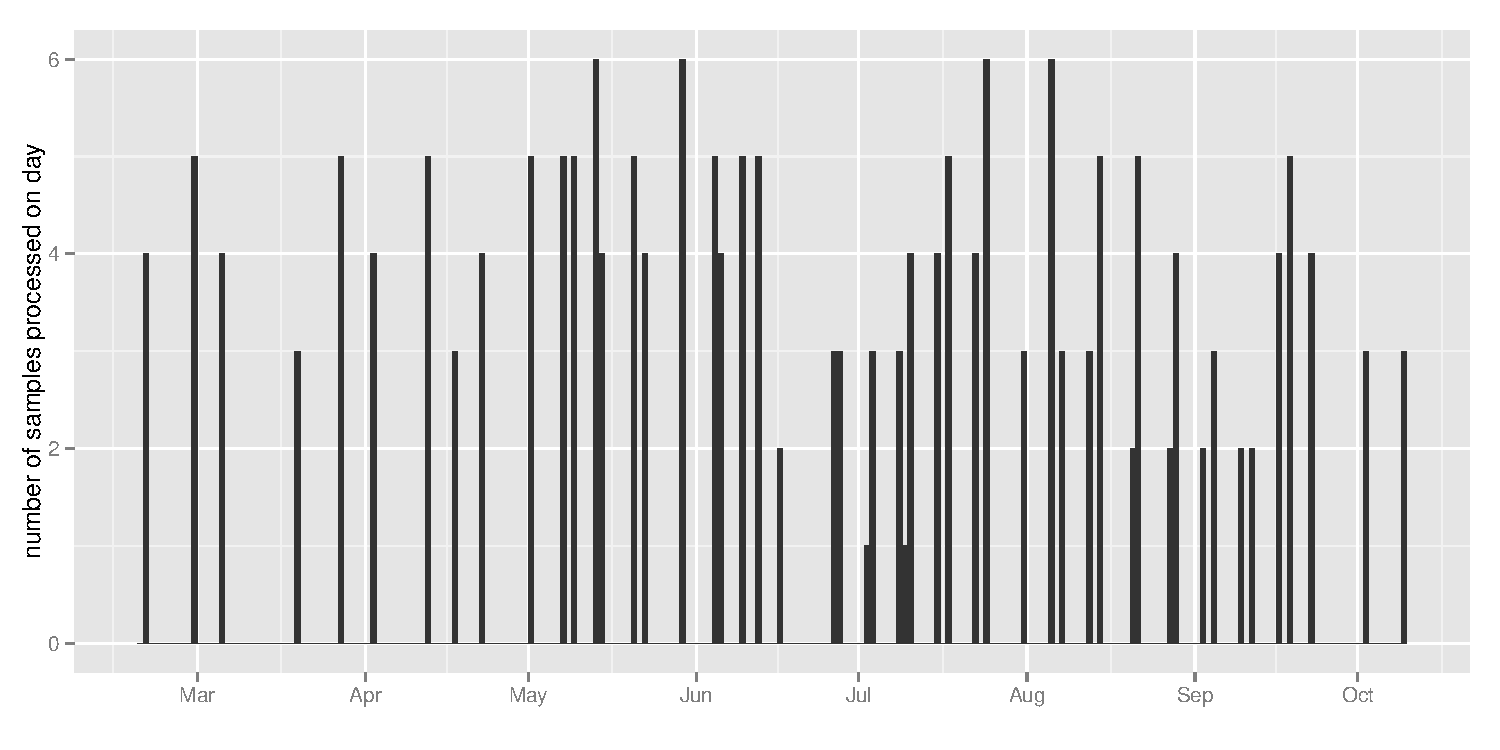
\includegraphics[scale=.5] {flowdatasets/figures/il2ra-samples-time.pdf}
\caption{
\label{figure:IL2RA-sample-time} 
}
\end{figure}


\begin{table}[ht]
\centering
\begin{tabular}{lllllll}
  \hline
         & individual & pch & day1       & day2       & day diff \\
  \hline
  1      & CB00058M   & a   & 2008-03-04 & 2008-09-16 & 196 \\
  2      & CB00427N   & b   & 2008-02-20 & 2008-10-02 & 225 \\
  3      & CB00435X   & c   & 2008-02-28 & 2008-10-02 & 217 \\
  4      & CB00459Y   & d   & 2008-03-26 & 2008-10-09 & 197 \\
  5      & CB00470K   & e   & 2008-04-10 & 2008-09-18 & 161 \\
  6      & CB00474P   & f   & 2008-04-16 & 2008-09-16 & 153 \\
  7      & CB00475Q   & g   & 2008-05-08 & 2008-09-18 & 133 \\
  8      & CB00496N   & h   & 2008-05-12 & 2008-09-22 & 133 \\
  9      & CB00503W   & i   & 2008-05-06 & 2008-09-18 & 135 \\
  10     & CB00555C   & j   & 2008-05-22 & 2008-09-16 & 117 \\
  11     & CB00563L   & k   & 2008-05-29 & 2008-09-18 & 112 \\
  12     & CB00566P   & l   & 2008-05-29 & 2008-09-18 & 112 \\
  13     & CB00568R   & m   & 2008-05-29 & 2008-09-22 & 116 \\
  14     & CB00588N   & n   & 2008-06-12 & 2008-10-09 & 119 \\
  15     & CB00591R   & o   & 2008-06-16 & 2008-09-22 & 98 \\
  16     & CB00646B   & p   & 2008-07-15 & 2008-10-02 & 79  \\
  \hline
\end{tabular}
\caption{ \label{table:IL2RA-recalled-individuals} Sixteen individuals recalled between 79 and 226 days later. }
\end{table}




\subsection{Manual Gating}






%\section{IL-2 stimulation}
%\input{flowdatasets/il2-stimulation.tex}
%\section{DILT1D}
%
\subsection{Panels}

\begin{table}[h!]\footnotesize
\begin{tabularx}{\textwidth}{cccccccc}
\rowcolor{Gray} 
CTLA-4 & CD69  & EFF   & TFH   & CD31  & NK    & intra FOXP3 & ex vivo \\
HLADR  & HLADR & CCR4  & PD-1  & CCR7  & CD56  & FOXP3       & FOXP3 \\
CD62L  & CD62L & CD62L & CD62L &       & CD161 & CD62L       & CD56 \\
CCR6   & CCR6  & CCR6  & CXCR5 & CD31  & TCRab & HELIOS      & pSTAT5 \\
CXCR3  & CXCR3 & CXCR3 & CXCR3 &       & CD69  & KI67        & \\
CTLA-4 & CD69  & CCR10 & ICOS  & CD122 & CD122 & CTLA-4      & \\
CD127  & CD127 & CD127 & CD127 & CD127 &       & CD127       & \\
CD25   & CD25  & CD25  & CD25  & CD25  & CD25  & CD25        & CD25 \\
CD4    & CD4   & CD4   & CD4   & CD4   & CD4   & CD4         & CD4 \\
CD8    & CD8   & CD8   & CD8   &       & CD8   & CD8         & CD8 \\
       &       &       &       & CD3   &       &             & CD3 \\
\end{tabularx}
\caption{ \label{DILT1D-panels}
The fluorochrome-antibody panels used in the DILT1D dataset.
}
\end{table}


\subsection{Samples}

35 subjects recalled up to 10 visits.

 
\chapter{ \label{appendix:fcs-data-format}Flow Cytometry Standard (FCS) Data Formats: FCS 2 vs FCS 3}

The objective of the Flow Cytometry Standard is to define a unified file format for flow data
that allows files created by one type of acquisition hardware and software to be analyzed by any other type.
The data format determines the range and the precision of the data stored.

The first Flow Cytometry Standard format for data files was FCS 1.0 \citep{Murphy:1984ev}.
The standard was later updated in 1990 as FCS 2.0 \citep{Anon:1990ce} and again in 1997 as FCS 3.0 \citep{Anonymous:vr}.
FCS 2.0 and FCS 3.0 are the current two main competing standards.


FCS 2 is a logarithmically compressed format which does not allow negative intensities.  
Instead negative values reported by the instrument are arbitrarily assigned the minimum value.
This leads to what is described as the log artefact: a pile up of intensities on the axes for low intensity values.
FCS2 data are integers in the range $1$ to $10000$ (4 decades).
FCS 3 on the other hand is closer to the raw data, covers a greater range and allows for negative values.
FCS 3 leaves more flexibility to the choice of transform.
FCS 3 are floating point numbers in the range $-211$ to $262143$ (8 decades)
FCS 2 is more trivial to process as it requires practically no post processing except for a log transform.
FCS 3 requires more careful thought as it leaves to us the compensation and the choice of a suitable transformation.
%In my work so far I have been using FCS 2 to facilitate comparison to the manual analysis but in the future I intend to use FCS 3 instead.  
%FCS 2 has compensation pre-applied whereas in FCS 3 compensation matrix is stored as part of the data format and needs to be applied manually.
%Unfortunately due to limitations of the fluorescent dyes and the instrument, the fluorescent signal measured in on channel is often a mixture of signals.
%This phenomenon is known as spectral spillover.
%The deconvolution of this signal is a process known as compensation.  The matrix solution is known as the spillover matrix
%and is usually a square matrix if there as many dyes as there are detectors.


 
\chapter{ \label{appendix:compensation} Compensation: accounting for fluorescent signal crosstalk in flow cytometry}

\begin{figure} [ht]
\begin{center}
   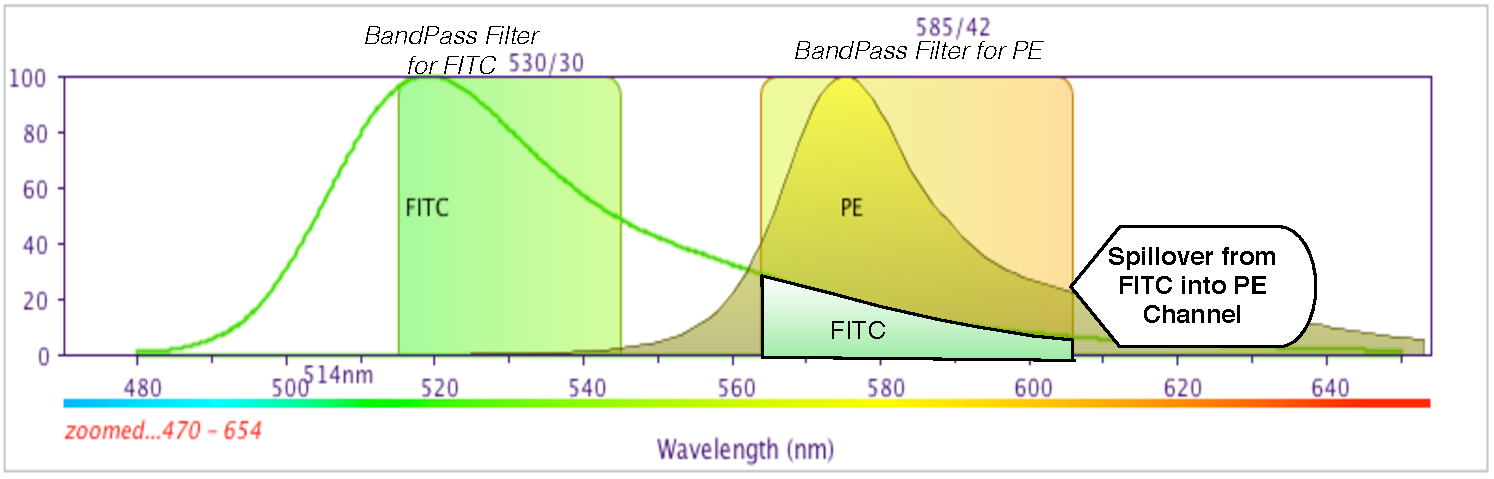
\includegraphics[scale=0.6]{introduction2/figures/spillover.pdf}
\end{center}
\mycaption{figure:spillover}
{ Leaking of signal from FITC fluorochrome into PE detector.}
{
  \small{Created using: \url{http://www.bdbiosciences.com/research/multicolor/spectrum_viewer/}}
}
\end{figure}

\begin{table}[ht]
\begin{center}
\begin{tabular}{rrrrrrr}
  \hline
%\backslashbox{Signal}{Detector} & Alexa-488 & PE-Cy7 & APC & PE & Alexa-700 & Pacific Blue \\ 
\backslashbox{Signal}{Detector} & PMT 1 & PMT 2 & PMT 3 & PMT 4 & PMT 5 & PMT 6 \\ 
  \hline
Alexa-488    & 100 &   0 &   0 &  16 &   0 &   0 \\
PE-Cy7       &   0 & 100 &   0 &   1 &   2 &   0 \\
APC          &   0 &   0 & 100 &   0 &  30 &   0 \\
PE           &   2 &   1 &   0 & 100 &   0 &   0 \\
Alexa-700    &   0 &   1 &   2 &   0 & 100 &   0 \\
Pacific Blue &   0 &   0 &   0 &   0 &   0 & 100 \\
   \hline
\end{tabular}
\end{center}
\mycaption{table:spillover}
{ Spillover matrix of the fluorochomes used by \citet{Dendrou:2009dv} obtained using single colour beads. }
{
Each entry is the percentage of the emitted fluorochrome signal (row) picked up by a detector (column).
The rows represent the fluorochomes and the columns are the PMT detectors.
Each detector is tuned to capture the intensity of a single fluorochrome (diagonal entries).
Spillover occurs when certain fluorochromes are detectable by more than one detector (non-zero terms off the diagonal).
Notice that there is non-negligeable spillover (\SI{30}{\percent}) of APC into PMT 5, the detector meant for Alexa-700.
}
\end{table}


%As we delve deeper into the lymphocyte subsets more fluorochromes are needed to further distinguish between different classes \citep{Perfetto:2004cy}.
%However when adding more and more fluorochromes, overlap of emission spectra becomes unavoidable.
%This implies that the intensity signal captured in a given detector is no longer originating from one single fluorochrome but is actually a combined signal emanating from multiple fluorochromes \citep{Roederer:2001vi}.
%To account and correct for this, the overlap needs to be assessed by evaluating the pairwise contribution of the signal of one fluorochrome to that of an other.
%These pairwise values can then be summarised in what is known as a spillover or compensation matrix (Table~\ref{table:spillover}).
%By subtracting the spillover values to the mixed intensity one can then recover the original intensity.
%This compensation step is usually performed after all the data from an experiment has been collected before commencing analysis.

As we delve deeper into the lymphocyte subsets more fluorochromes are needed to further distinguish between different classes \citep{Perfetto:2004cy}.
However when adding more and more fluorochromes, overlap of emission spectra becomes unavoidable \citep{Roederer:2001vi}.
%This implies that the intensity signal captured in a given detector is no longer originating from one single fluorochrome but is actually a combined signal emanating from multiple fluorochromes \citep{Roederer:2001vi}.
This implies that the intensity signal measured in one detector is in fact a mixture of signals from other flurochromes which spillover across detectors (Figure~\ref{figure:spillover}).
The deconvolution of this signal is a process known as compensation.
The matrix solution is known as the spillover matrix and is usually a square matrix with as many rows as there are fluorochromes and columns as there are detectors
%if there as many dyes as there are detectors 
(Table~\ref{table:spillover}).
To calculate the spillover matrix single coloured beads are used. 
The pairwise contribution of a fluorochrome to a non-specific channel is then summarised in a compensation matrix.
%To account and correct for this, the overlap needs to be assessed by evaluating the pairwise contribution of the signal of one fluorochrome to that of an other.
%These pairwise values can then be summarised in what is known as a spillover or compensation matrix (Table\ref{table:spillover}).

%This phenomenon is known as spectral spillover.

By subtracting the spillover values from the mixed intensity one can then recover the original intensity.

This compensation step is usually performed after all the data from an experiment has been collected before commencing analysis.


 
\chapter{\label{appendix:transformation}Data transformations: Rescaling Data for Display and Analysis}


As fluorescence intensity tends to scale multiplicatively, intensity data needs to be linearised for the purpose of visualisation and clustering.
Clustering algorithms based on variance (average distance to the mean) perform poorly on skewed data. 

%Given a finite range (number of channels/bins), a logarithmic transform can be used to maximise the range of data that can be captured by a detector.

Given FCS 2 data is strictly positive, a simple $\log_{10}$ transform is usually applied.
However FCS 3 allows negative values so an offset parameter $b$ may be specified:
\[
    f(x) = \log_{10}(x+b)
\]
However for low and negative intensities, a linear transform is preferred to a logarithmic transform \citep{Tung:2006uw} as it is less distortive.
%this transform distorts the data: it shrinks the distance between points making clusters less distinguishable
Some more appropriate transformations for FCS 3 are the Generalized Arcsinh, the Biexponential, the LinLog and the Generalized BoxCox
\citep{Bagwell:2005he,Parks:2006gaa,Finak:2010is}.
Given the data, parameters for these transformations can be estimated using maximum likelihood assuming a multivariate Gaussian distribution of the data \citep{Finak:2010is}. 

%assume a global distance metric.
%as illustrated in Figure~\ref{figure:transform}.
%One issue in choosing a transform is whether to allow for negative values.
%The simplest transform which can cater for negative values is a log transform with an offset parameter:

% Another possibility is the arcsinh transform which allows for negative values without requiring an offset to be specified:
%\[
    %f(x) = \operatorname{arcsinh}(x) = \log( x^2 + \sqrt { 1+ x^2 } )
%\]

%For the purpose of gating the bead data, the transform chosen for FCS2.0 data is a standard log transform (offset $b=0$)
%whereas for FCS3.0 we use an offset $b=50$ so to make all values positive:
%\[
    %f(x) = log(x+50)
But, as illustrated by \citet{Tung:2006uw}, care needs to be taken in choosing a suitable transform, as the choice of the parameters
infuences the shape of the distribution and can introduce extra modes.
Figure~\ref{figure:log10-transform} illustrates this phenomenon in our data when we apply the $Log_{10}$ transform.
Instead if we apply the logicle transform as defined by \citet{Parks:2006gaa} in Figure~\ref{figure:logicle-transform}, we see that we can address the spurious mode
by reducing the w parameter which represents the slope of the linear transform around zero.

%Update for the Logicle Data Scale Including Operational Code Implementations \citet{Moore:2012gz}

\begin{figure}
\centering
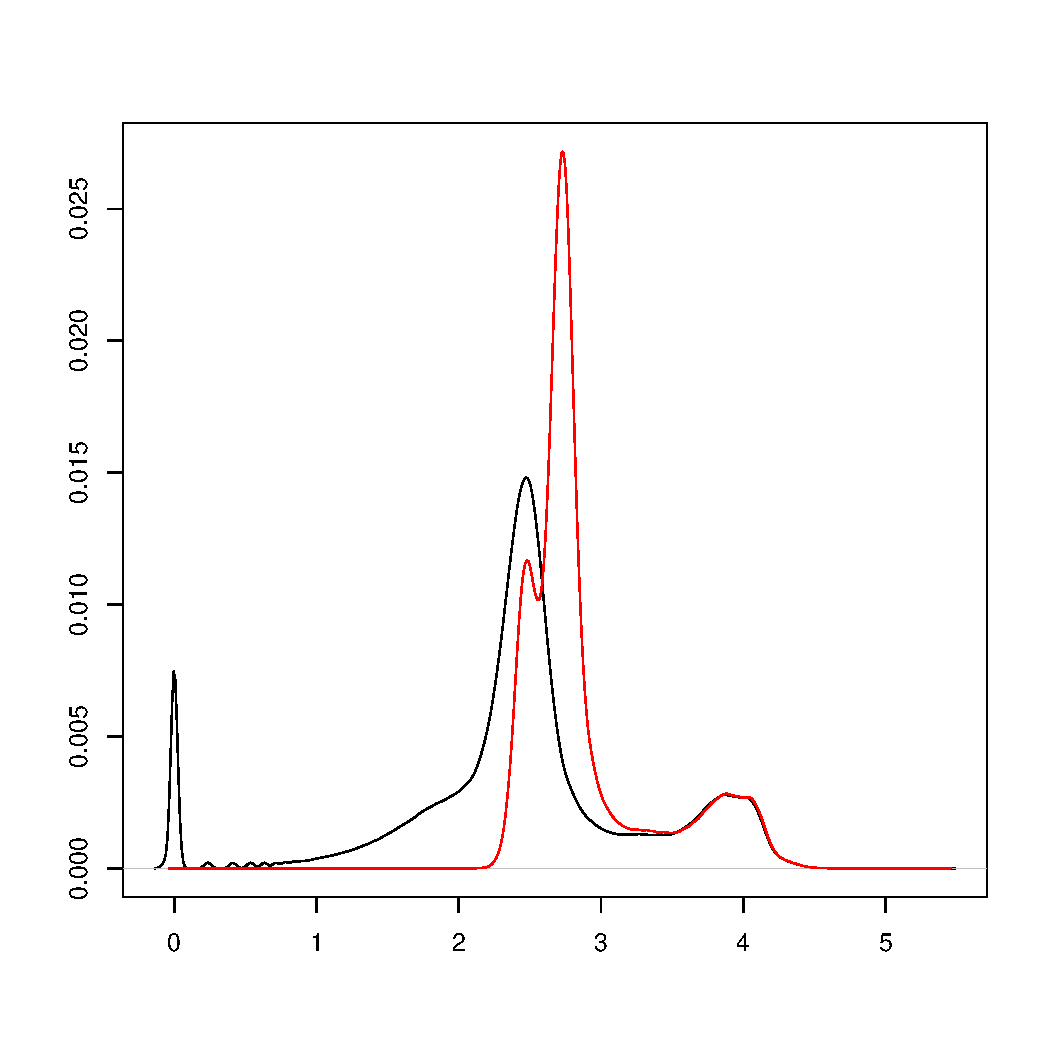
\includegraphics[scale=.5] {Appendix/figures/log10-transform.pdf}
\mycaption{figure:log10-transform} 
{$Log_{10}$ transformed data}
{
  In black, intensity values of zero or less are assigned to 1.
  In red, the intensity value are shifted by the minimum so that all negative values are greater than zero.
}
\end{figure}


\begin{figure}
\centering
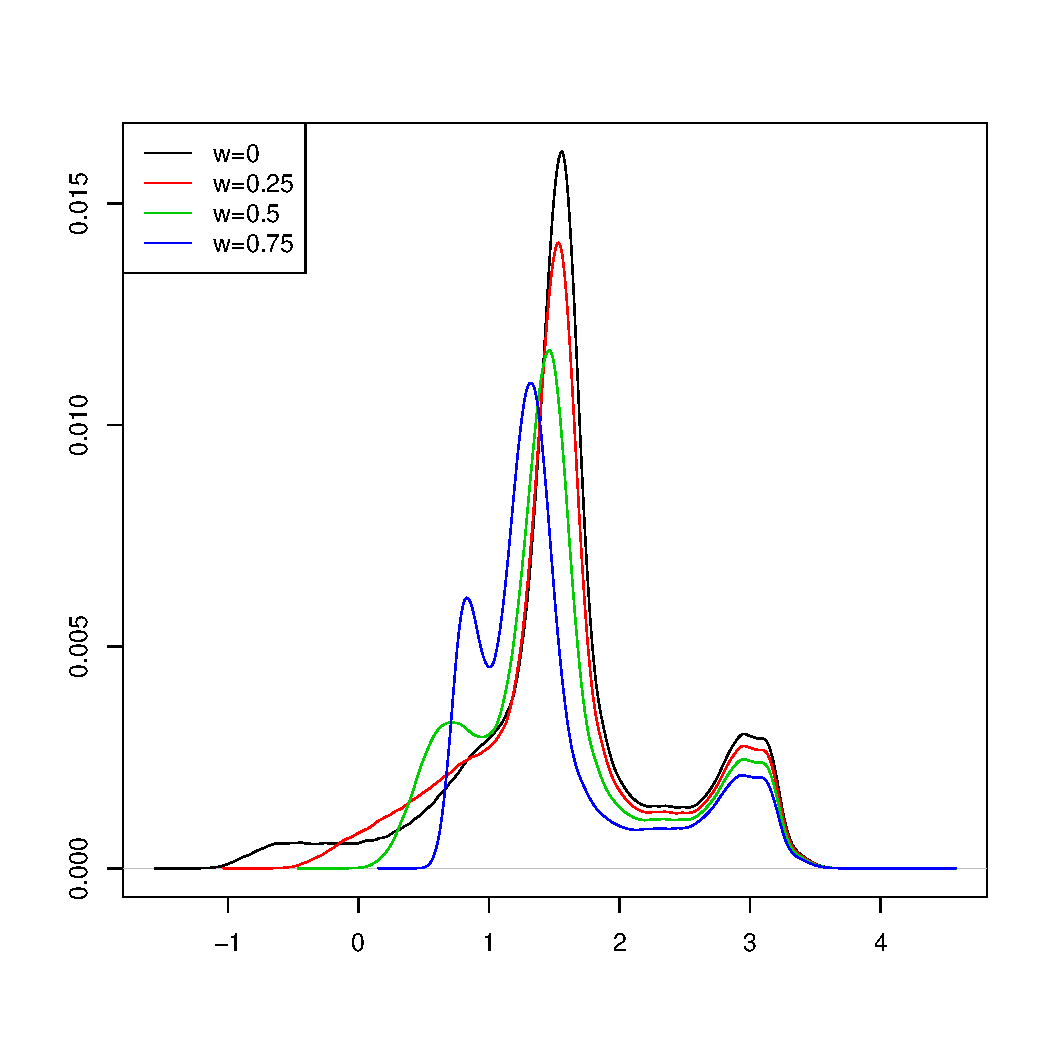
\includegraphics[scale=.5] {Appendix/figures/logicle-transform.pdf}
\mycaption{figure:logicle-transform} 
{$logicle$ transformed data}
{
  The logicle transform is similar to a logistic function in that it approximates a linear transform around the first decade
  and a log transform elsewhere.
  As w, the slope of the linear transform, increases the shape of the distribution approximates the shifted log transform in Figure~\ref{figure:log10-transform}.
}
\end{figure}



\chapter{ \label{appendix:normalisation} Normalisation and univariate clustering}

%The aim of this chapter is to give an overview of univariate normalisation methods.
%These methods are illustrated on simulated and real biological datasets.
%These methods can be generalised to multivariate datasets if ind

The purpose of normalisation is to remove unwanted experimental variation to make data comparable even when the samples are
collected on different days, processed with different protocols or instrumental configurations.
However distinguishing between unwanted and biological variation necessitates some prior knowledge about the datasets, either in the form of distributional assumptions
or of features which exist across samples.
Such features can then be used as reference points to normalise across samples.
If the features are modes in the data, then normalisation is equivalent to doing clustering, in order to identify the modes,
followed by meta-clustering to match the modes across samples.
In microarray gene epxression datasets, for example, one distributional assumption is that the majority of genes are not differentially expressed between samples from
similar tissue types.
The underlying principle is that true biological variation is specific whereas experimental variation affects the sample as a whole.

%The objective of flow cytometry is to capture variation in the biological sample not variation linked to the instrument or to other experimental factors.
%Normalisation is the process of factoring out non-biological for sensible comparison fo samples analysed at different times or on different instruments.

%Generally, samples obtained under controlled conditions should be sufficiently similar and variation in the whole sample is due to experimental artifact.
%Which is why normalisation should be done on the whole sample rather than a subset of the sample.

%The idea follows from gene MA that overall gene expression obtained under similar conditions should be quite similar.
%Hence normalisation in flow cytometry should be done on the whole sample (before any subsetting takes place).

%As datasets get larger they get more similar
%on a large scale things are quite similar but as we dig deeper into subsets distributions look different
%Or that the p-values in a GWAS should follow some empirical distribution.
%We will see that different normalisation approaches make different assumptions about what is unwanted variation.

%\section{Data sets} 
%\paragraph{KIR copy number} 
%\paragraph{Flow data}

\section{Data driven normalisation}

Perhaps the most basic form of normalisation is scaling: we substract the mean and divide by the variance so that the resulting distribution has a mean of zero and a variance of one.
%This approach is sensible if the distibutions are symmetric unimodal like the normal distribution.
Figure~\ref{normalisation-scaled} is a trivial example of scaling on simulated data.
%$x_0 \sim N

%% Scaling
\begin{figure}[ht]
\begin{subfigure}[b]{.5\textwidth}
\centering
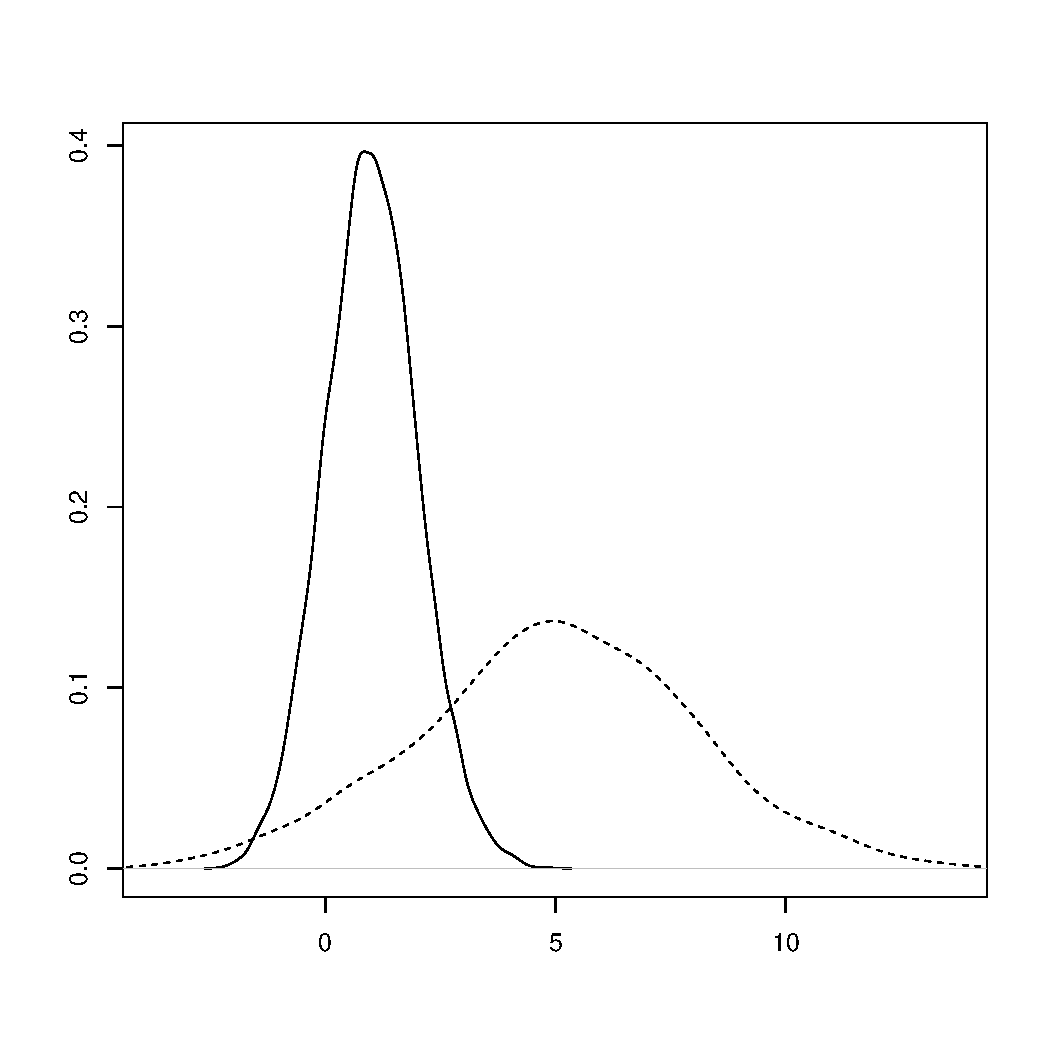
\includegraphics[scale=.4]{figures/normalisation-scaled-a.pdf} 
\caption{before scaling}
\end{subfigure}
~
\begin{subfigure}[b]{.5\textwidth}
\centering
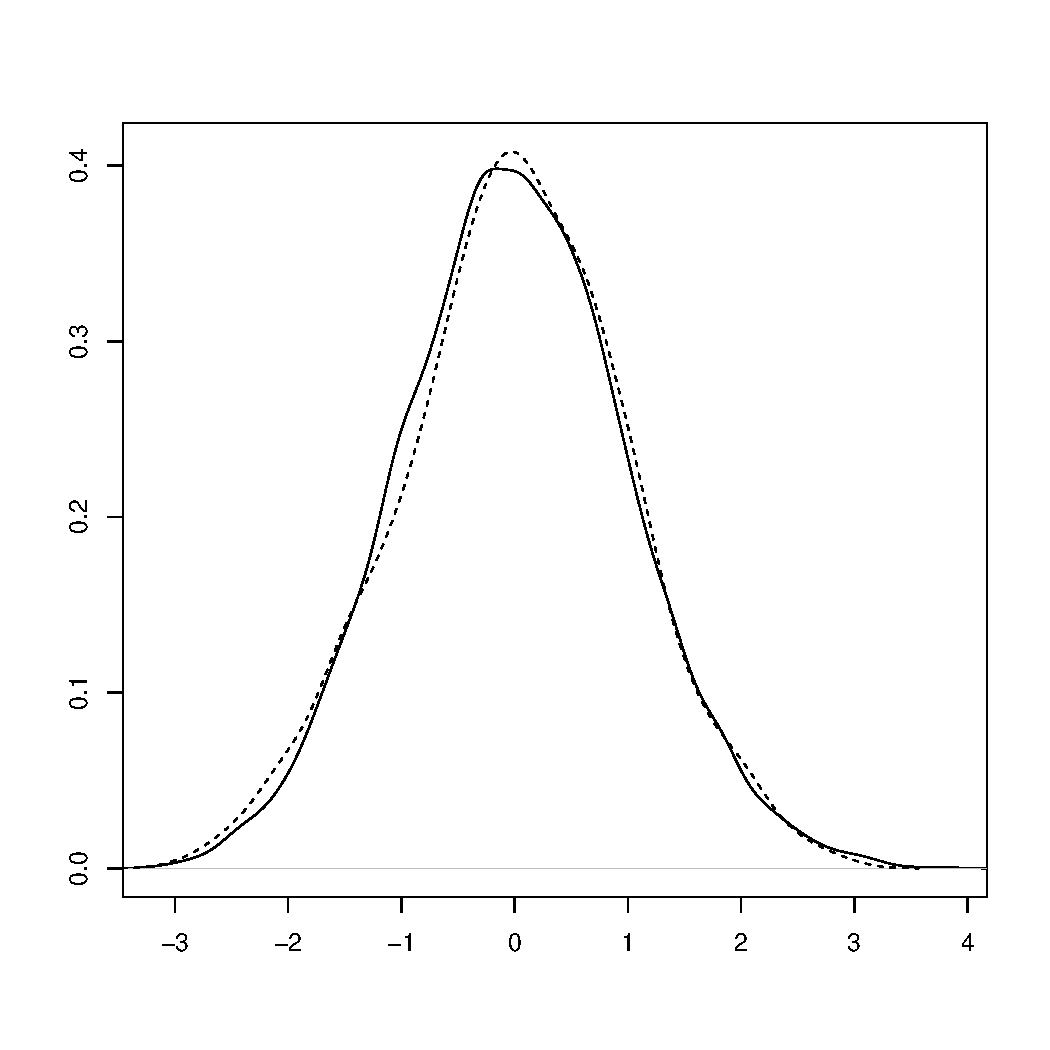
\includegraphics[scale=.4]{figures/normalisation-scaled-b.pdf} 
\caption{after scaling}
\end{subfigure}
\caption{ \label{normalisation-scaled}
In solid black line represents the density function obtained from $10,000$ draws from a normal distribution
with with means $\mu_0=1$ and standard deviation $\sigma_0=1$.
The dashed line represents the density function obtained from $1,000$ draws from a normal distribution
where $\mu_1=5$ and $\sigma_1=3$.
After scaling both distributions have $\mu=0$ and $\sigma=1$.
}
\end{figure}


If the distributions are unimodal but not symmetric, such as $\chi^2$ distributions, then an alternative is quantile normalisation.
As can be seen in Figure~\ref{normalisation-quantile}, the quantiles of the distribution are identified
then a transform is applied so that quantiles of one distribution are aligned with those of the other.
Here the transform is a simple linear regression.
Quantile normalisation works well when the shape of the distributions is the same and only shifted.

%% Quantile
\begin{figure}[ht]
\begin{subfigure}[b]{.5\textwidth}
\centering
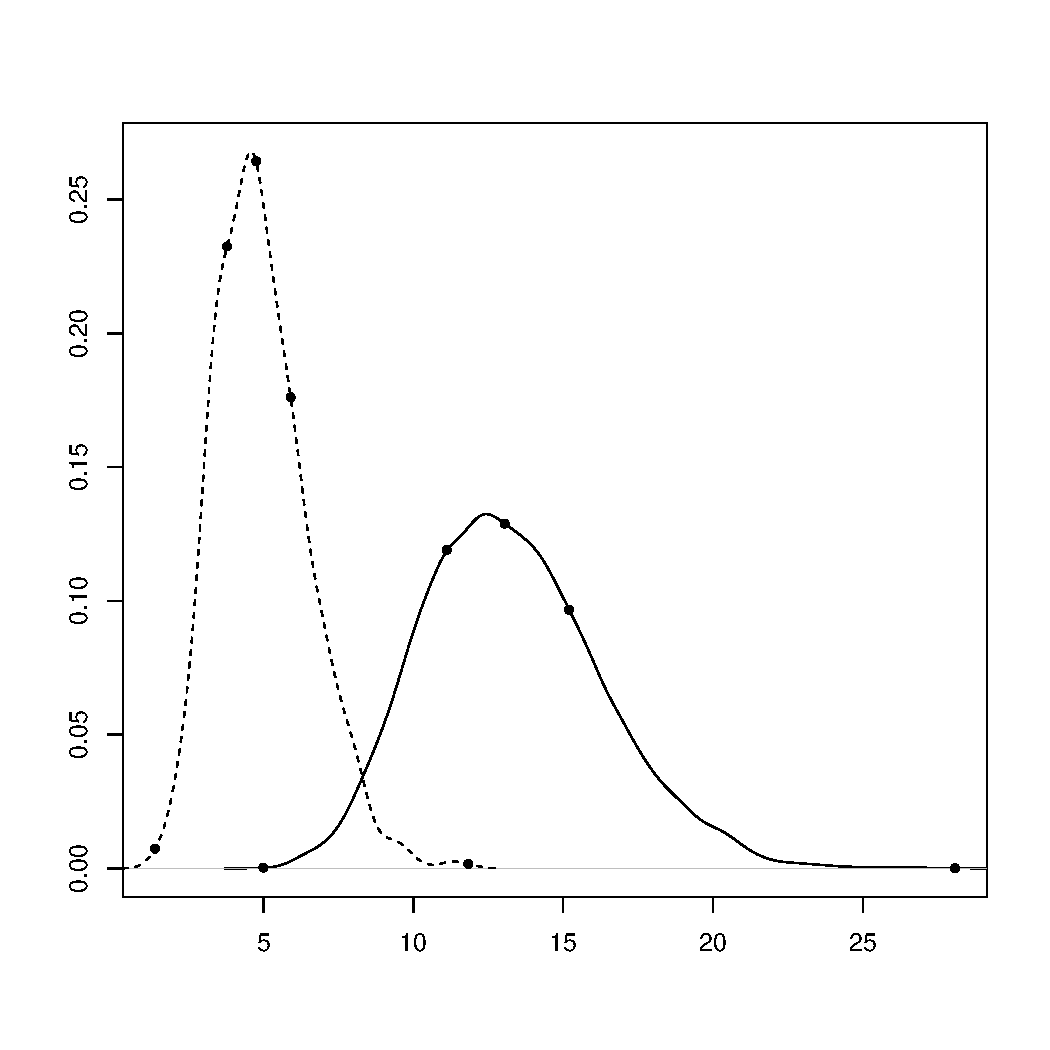
\includegraphics[scale=.4]{figures/normalisation-quantile-a.pdf} 
\caption{before aligning quantiles}
\end{subfigure}
~
\begin{subfigure}[b]{.5\textwidth}
\centering
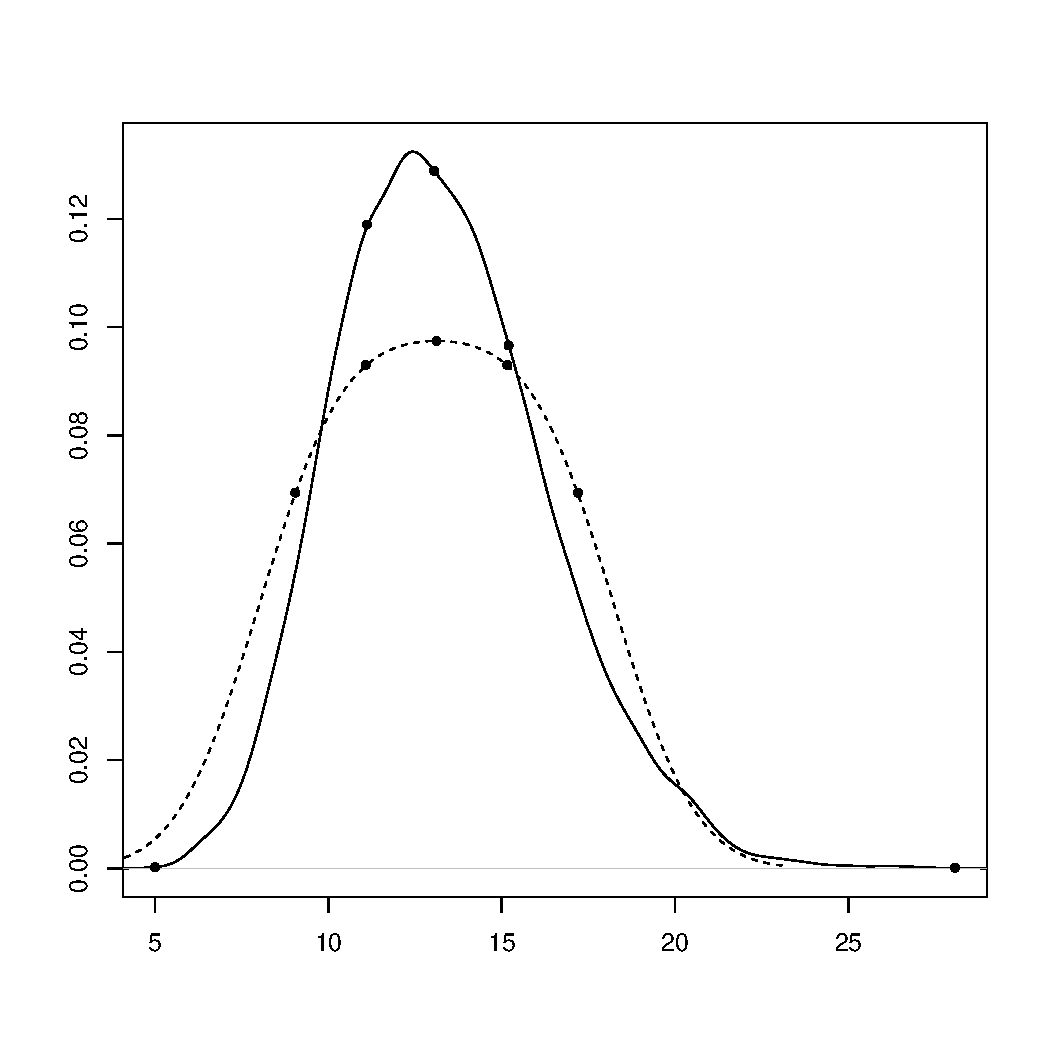
\includegraphics[scale=.4]{figures/normalisation-quantile-b.pdf} 
\caption{after aligning quantiles}
\end{subfigure}
\caption{ \label{normalisation-quantile}
In solid black line represents the density function obtained from $10,000$ draws from a gamma distribution
with with shape $\alpha_0=20$ and rate $\beta_0=1.5$.
The dashed line represents the density function obtained from $1,000$ draws from a gamma distribution
where $\alpha_1=10$ and $\beta_1=2$.
The black dots are the quantiles.
The normalisation finds a linear mapping of the quantiles of the dashed-line distribution onto those of the solid-line distribution.
}
\end{figure}


In real datasets however, univariate distributions are typically multimodal since they contain of a mixture of groups.
In the case of flow cytometry data, the groups are cell populations, and the modes of the distributions, esentially peaks in the density function,
represent the protein quantity carried on the surface of different cell types.
In theory, the locations of these peaks should remain fairly stable across samples provided experimental parameters are kept constant.
Though, in practise there is variation attributed to factors which are beyond our control such as long-term instrument deterioration.
On the other hand, the height of the peaks, the relative frequencies of the cell populations, are expected to change since they are
are susceptible to variation.
%In the case of qPCR data, the groups are reprentative of the copy numbers.

In such a scenario, a reasonable normalisation method is to align the peaks of the distributions so that different cell populations are centered
in a similar location across samples even when their relative quantity changes.
The implementation of this normalisation method then depends on the method used to identify the peaks and to match them across samples.

The ideal scenario is when the number of peaks is known and constant across samples.
This is the case when dealing with synthetic data such as beads.
In this scenario, basic clustering algorithms such as k-means or k-medoids, can be applied to identify the peaks in each sample.
This is the method used by the \Rpackage{flowBeads} BioConductor package which identifies bead populations with the k-medoids algorithm
for the purpose of fluorescence normalisation.

Unfortunately, on real data, the uncontrolled variation between biological samples means that the certain peaks are not consistently identifiable across all samples.
The number of peaks is unknown and can vary between samples. 
More flexible peak searching algorithms are requied to allow for this per sample-variation.

Instead of clustering, another method is to identify peaks in the density function with a sliding window approach.
The sliding window approach records the point with the highest density estimate in the current window.
As a result returning a list of highest density points of which the top K may be chosen.
This is one of the approaches implemented in the \Rpackage{flowStats} BioConductor package.
Here's an example of this method applied on flow data where two common groups stand out and are reasonably well separated (Figure~\ref{figure:normalisation-peaks}).

Sometimes it may be preferable to identify only the most distinguishable subset of peaks, those representative of the most common groups.
This is the method we applied on qPCR data to align common copy number groups 1 and 2 across plates.
%However peaks are not always easily identifiable.


%% Peaks
\begin{figure}[ht]
\begin{subfigure}[b]{.5\textwidth}
\centering
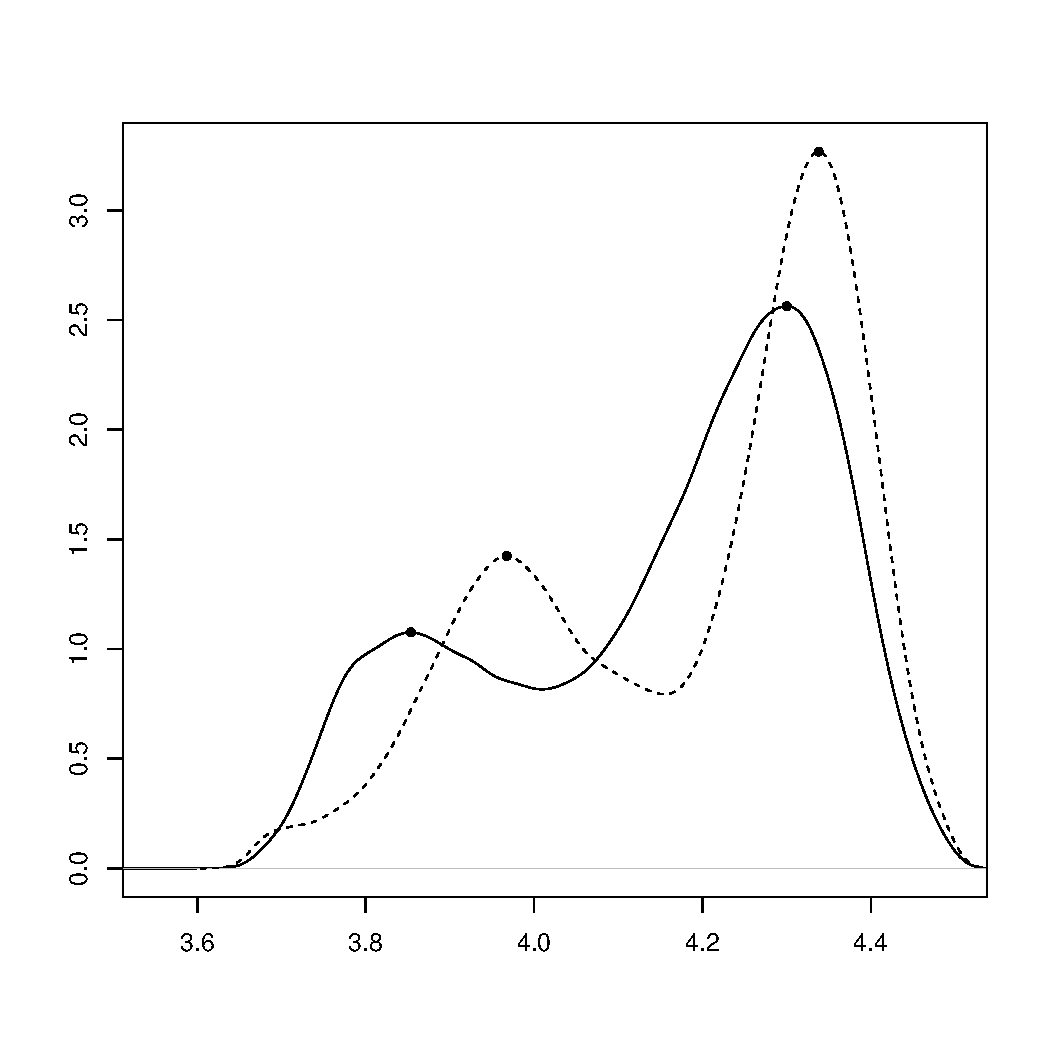
\includegraphics[scale=.4]{figures/normalisation-peaks-a.pdf} 
\caption{identification of peaks}
\end{subfigure}
~
\begin{subfigure}[b]{.5\textwidth}
\centering
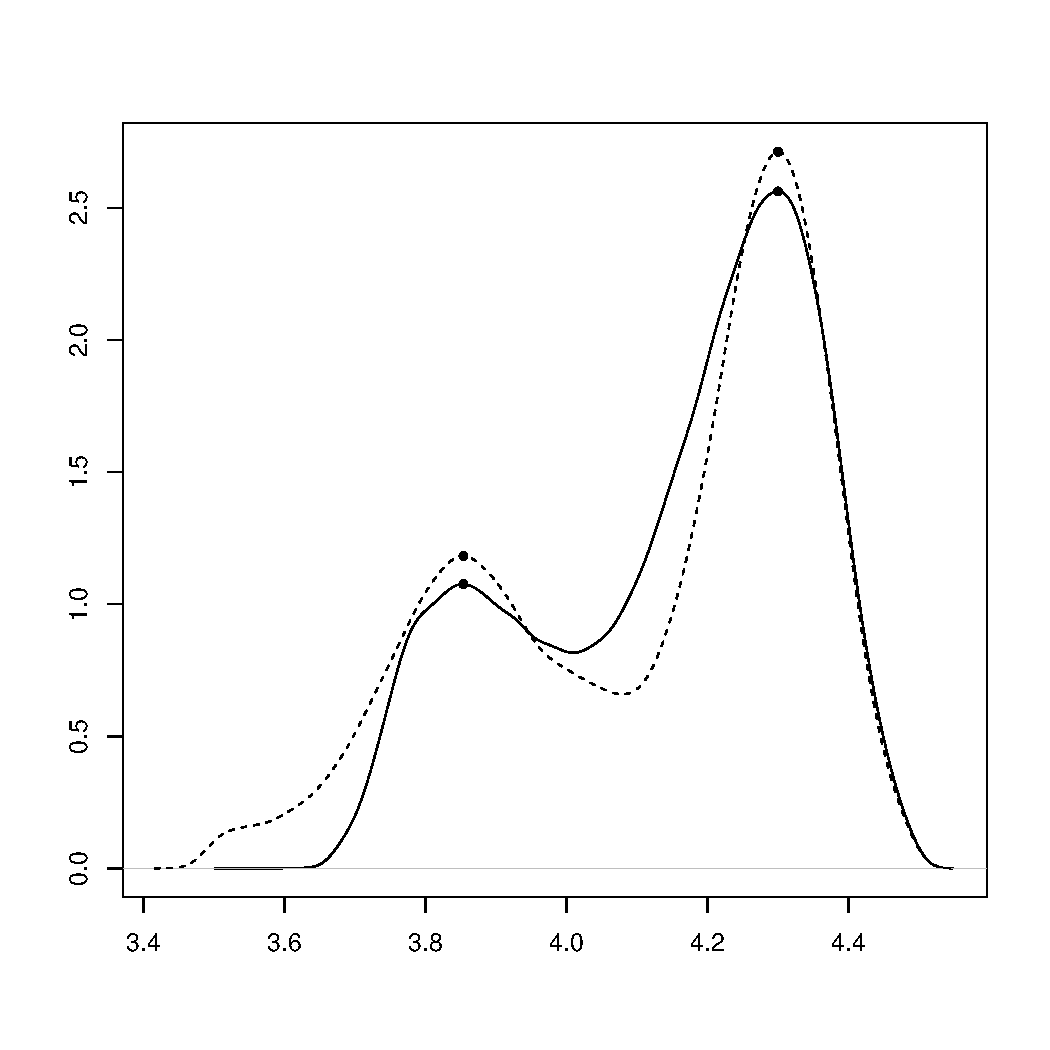
\includegraphics[scale=.4]{figures/normalisation-peaks-b.pdf} 
\caption{peak alignment}
\end{subfigure}
\caption{ \label{normalisation-peaks}
Alignment of the two identified peaks.
}
\end{figure}


These break down into three steps.
First feature are identified within each sample.
Then the features are matched across samples.
Finally the features are aligned across samples using a transform which
may be linear on non-linear.
This last step represents the actual normalisation step.

\subsection{Identification of features within a sample}

Feature identification can work directly on the data, by doing clustering,
or on the shape of the univariate density function.  
The shape and smoothness of the density function is determined by the choice of bandwidth.
Hence these methods which work directly on the density function are sensitive to the bandwidth selection (also known as the smoothing parameter).

\textbf{Sliding-window on the density function}
In the sliding-window approach, when the maximum of the window coincides with the central data point of the window, 
this data point is assigned to be the maximum.
This is the approach adopted by the \Rfunction{guaussNorm} function in \Rpackage{flowStats}.
This method is dependent on the span of the sliding-window.
Peaks are also scored depending on their height and peakness.
This allows for a ranking of the peaks by quality.
I have applied this sliding-window method with a fixed window size of 40 to all three available flow datasets in Figure~\ref{figure:IL2-density-peaks},
Figure~\ref{figure:IL2RA-density-peaks} and Figure~\ref{figure:DILT1D-EFF-density-peaks}.
No attempt has been done to rank the peaks by score, instead the peaks are ordered by their location.
The coloured points represent the peaks identified in each sample.
The colours determine the ordering of the peaks: black, red, green, blue, light-blue.
The success of the peak identification varies greatly between channels.
When the number of peaks identified is not consistent, we see a mixing of the colours.
Sometimes a consensus can be determined from considering all sample.
For example for CD4 in Figure~\ref{figure:IL2-density-peaks}, it is clear
that the correct number of peaks in the majority of samples should be four even when sometimes the first peak is not consistently detected
in a few sample.
On the other hand, in CD45RA of the same figure, it is unclear whether there should be two or three peaks.
Here we might try to use the score of the peaks to decide of where the should peak should lie.


\begin{figure}[h]
  \centering
  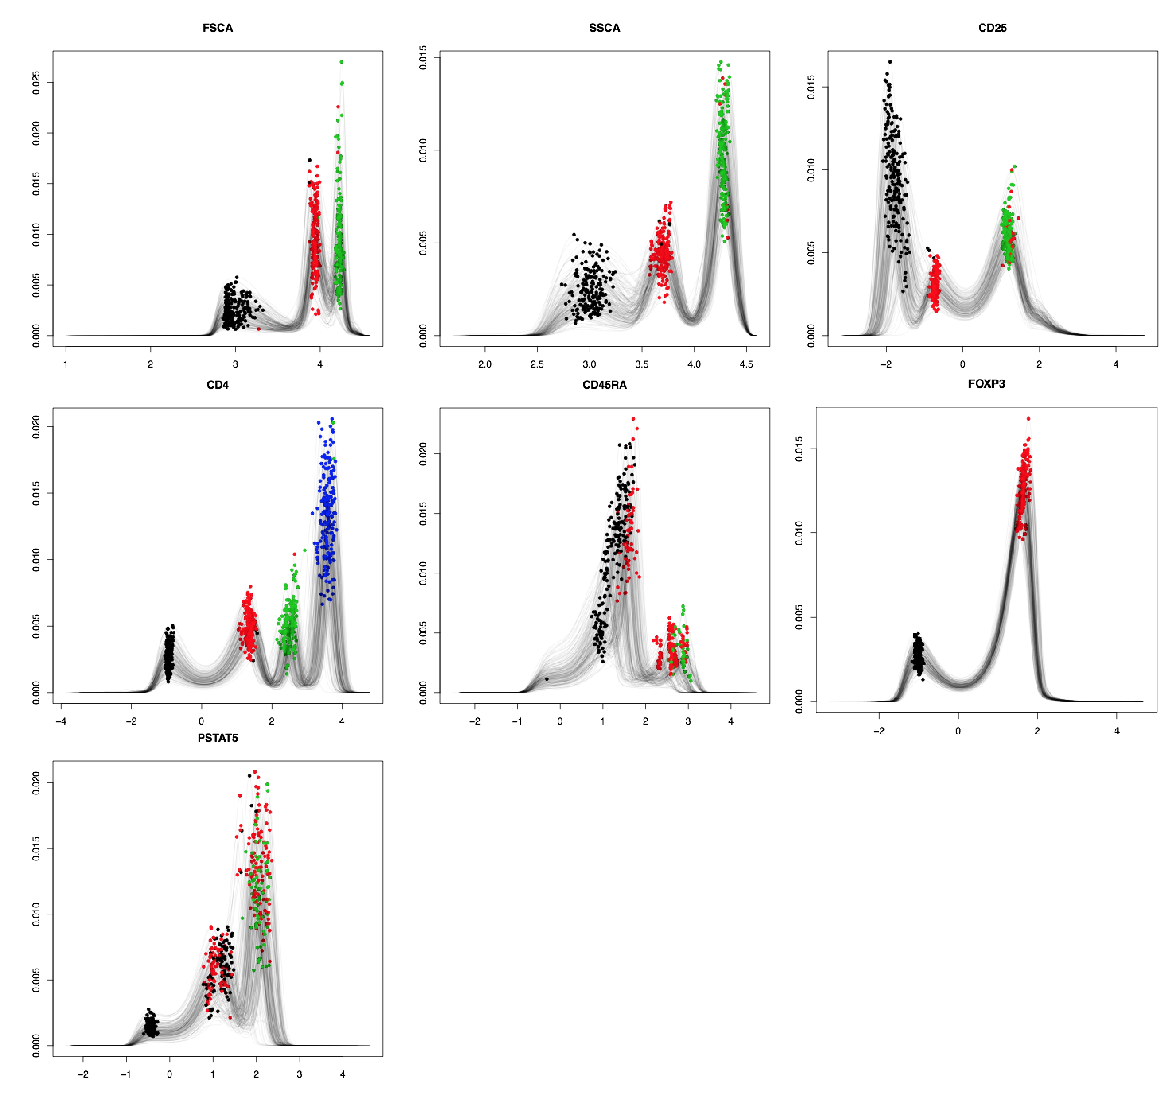
\includegraphics[scale=.75]{figures/IL2-density-peaks.pdf}
  \mycaption{figure:IL2-density-peaks}{IL-2 stimulation dataset, sliding-window span $40$.}{  
  The coloured points indicate the peaks as identified by the sliding window approach with a window span of 40.
  The colouring indicate the number of the peak. The respective ordering for four peaks is black, red, green, blue.
  Notice that often there is mixing of the colours.
  This happens because the same number peaks is not always identified depending on the sample and window size.
  In fact certain peaks can not be reliably identified such as on pSTAT5.
}
\end{figure}


\begin{figure}[h]
  \centering
  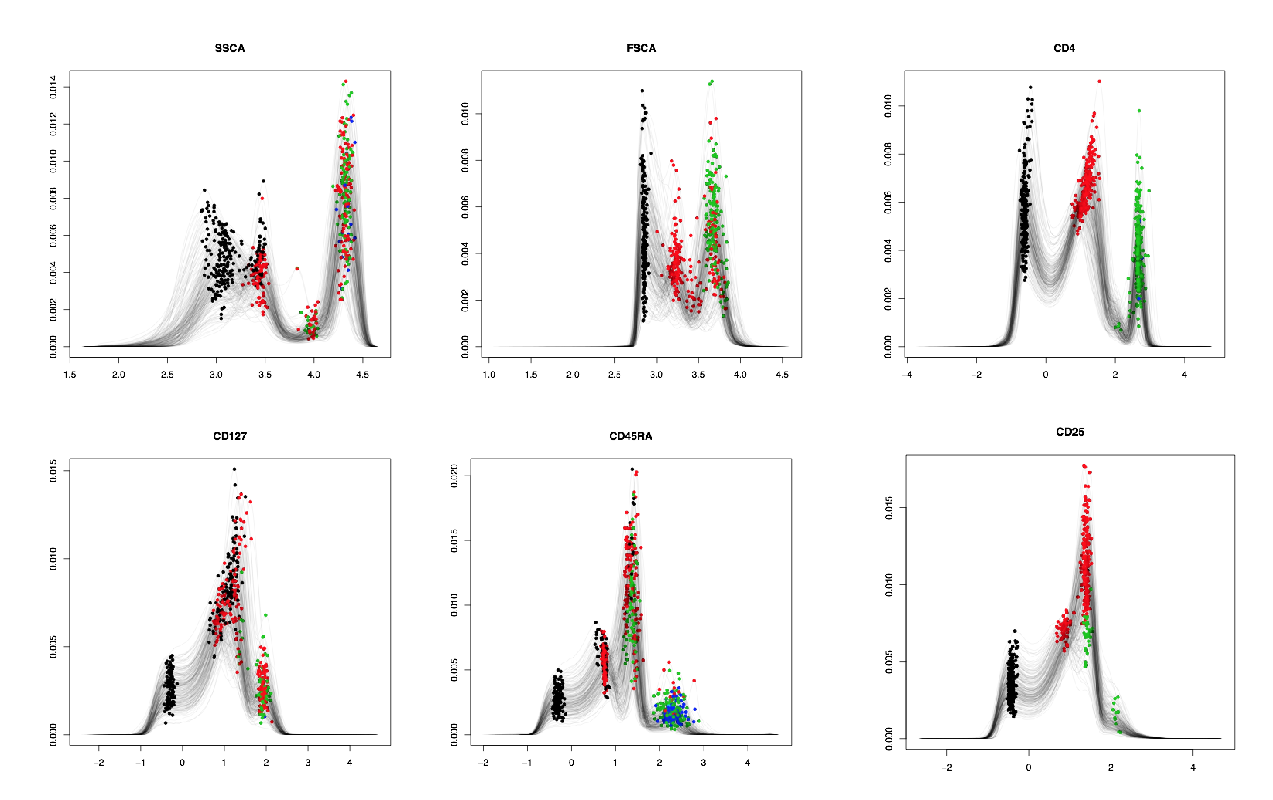
\includegraphics[scale=.75]{figures/IL2RA-density-peaks.pdf}
  \mycaption{figure:IL2RA-density-peaks}{IL2RA dataset, sliding-window span $40$.}{
  The coloured points indicate the peaks as identified by the sliding window approach with a window span of 40.
  The colouring indicate the number of the peak. The respective ordering for four peaks is black, red, green, blue.
  Notice that often there is mixing of the colours.
  This happens because the same number peaks is not always identified depending on the sample and window size.
  In fact certain peaks can not be reliably identified such as on pSTAT5.
  }
\end{figure}


\begin{figure}[h]
  \centering
  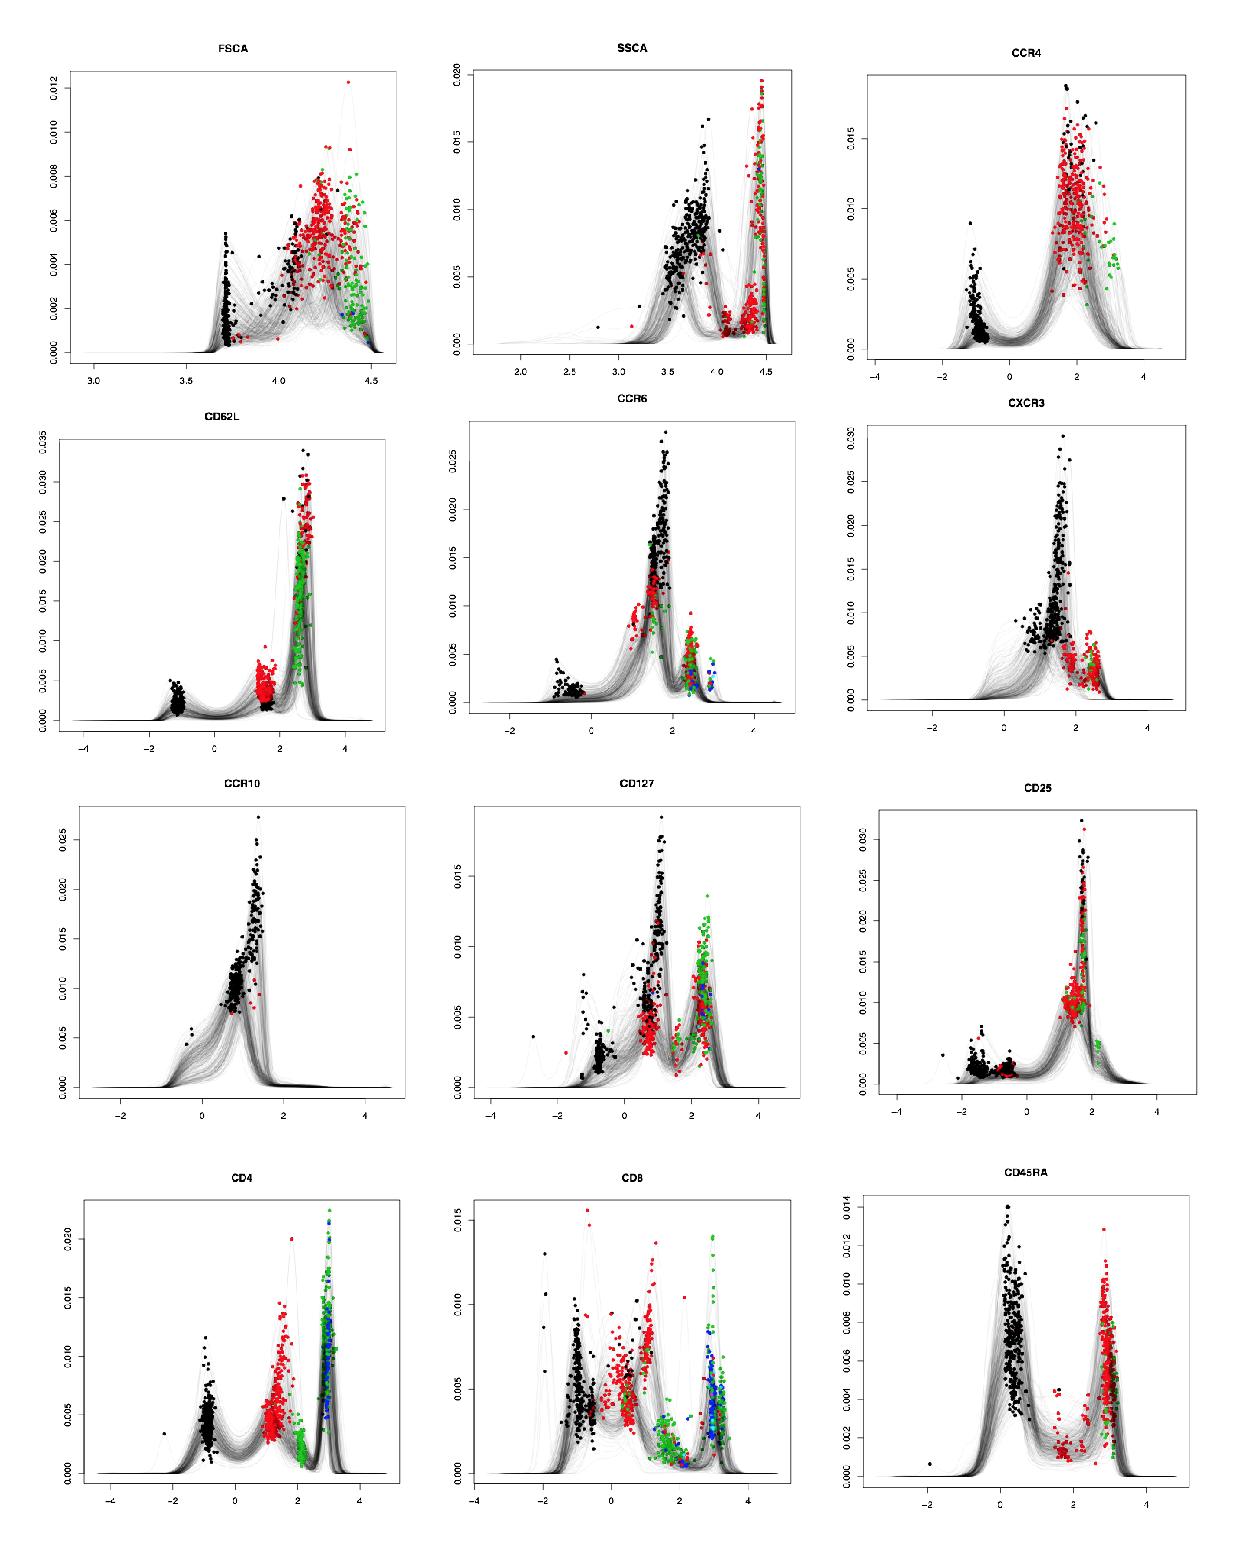
\includegraphics[scale=.75]{figures/DILT1D-EFF-density-peaks.pdf}
  \mycaption{figure:DILT1D-EFF-density-peaks}{DILT1D dataset, sliding-window span $40$.}{
  The coloured points indicate the peaks as identified by the sliding window approach with a window span of 40.
  The colouring indicate the number of the peak. The respective ordering for four peaks is black, red, green, blue.
  Notice that often there is mixing of the colours.
  This happens because the same number peaks is not always identified depending on the sample and window size.
  In fact certain peaks can not be reliably identified such as on pSTAT5.
}
\end{figure}


\clearpage


\paragraph{Feature signifance of the density function}

%The reliance on the bandwidth by trying a selection of bandwidths.
Another approach is to estimate feature significance using the gradient and curvature kernel density estimation \citep{Chaudhuri:1999gu,Duong:2008eu}.
%SiZer: significant zero crossing of derivatives

This approach as implemented by \Rfunction{featureSignif} in the \Rpackage{feature} R package, relies on a $\chi^2$ significance test.

Feature identification uses the first (gradient) and second derivate (curvature) of the density function to identify features such as local maxima, minima or points of inflection.
Local maxima are points where the first derivative is zero and the second derivative is strictly negative.
Local minima are ponts where the first derivative is zero and the seoncd derivative is strictly positive.
%When both the first and second derivative are zero then it's a point of inflection.

In practise however this method does not reliably identify peaks.
Possibly, the bandwidth and threshold significance threshold selection require better estimation.


\paragraph{Clustering}
Peaks in the density function can be also identified without explicitly analysing the density function but instead by using data clustering.
These methods are sensitive to the number of clusters parameters which, as mentionned, may not always be consistently identifiable across samples.
Perhaps the number of cluster can be estimated from the sliding window results obtained on all samples.

The most fundamental and well known univariate clustering algorithm is K-means (see Appendix\ref{appendix:clustering}).


\subsection{Feature matching across samples }

Feature matching, also called feature registration, attempts to match the identified features across samples.
This is similar to a meta-clustering step.
Samples may have different number of features.
Density features can be matched on properties such location and height.
Clusters can be matched using position or size of group.
Consensus about the number of groups common to all samples.


\subsection{Alignment of features across samples}

Methods which attempt to align the features/landmarks of the density functions via some linear or non-linear transform \citep{Hahne:2009hl}.

Once the peaks have been identified a transform can then be defined so that they are aligned across samples.
If there are only two peaks, then a linear transform perfectly aligns the two peaks.
But if there are more than two peaks, alignment could necessitate a non-linear transform.
However this runs the risk of introducing too much extra-variation in the dataset.
%The shifting of the data of the data can be done using a linear transform which scales the variance by the slope squared.

\paragraph{Linear}

Linear regression preserves variance.
But certain peaks which are far from the mean have more leverage.
Peaks may be weighted by their height, since more significant should be attributed more weight.


\paragraph{Non-linear}

In the \Rpackage{flowStats}, two methods non-linear are suggested: \Rfunction{gaussNorm} and \Rfunction{fdaNorm}.

In the \Rfunction{gaussNorm} approach, the amount by which the data points are shifted is exponentially decreased as the points are further away from the features.
Thus features can be moved independently from each other.

In the \Rfunction{fdaNorm} approach, after approximating the density function with b-splines and identifying features, a warping function is used to transform the curves.
This is also known as curve registration and is implemented in the fda R package.

Another non-linear regression approach is local regression.

The loess approach uses locally weighted polynomial

At each point in the data set a low-degree polynomial is fitted to a subset of the data, with explanatory variable values near the point whose response is being estimated.
The polynomial is fitted using weighted least squares, giving more weight to points near the point whose response is being estimated and less weight to points further away.
The value of the regression function for the point is then obtained by evaluating the local polynomial using the explanatory variable values for that data point.
The loess fit is complete after regression function values have been computed for each of the n data points.

Many of the details of this method, such as the degree of the polynomial model and the weights, are flexible.


%\begin{figure}[h]
%%
%%#simulated data
%%x0 <- mixtools::rnormmix(1000, mu=c(1,6), lambda=c(.3,.7))
%%x1 <- mixtools::rnormmix(1000, mu=.9*c(1,6)+2, lambda=c(.5,.5), sigma=c(2,2))
%%d0 <- density(x0)
%%d1 <- density(x1)
%%l0 <- extract.landmarks(x0,max.lms=2, bw=d0$bw)
%%l1 <- extract.landmarks(x1,max.lms=2, bw=d1$bw)
%%m <- lm(l0$lms ~ l1$lms)
%%x1.norm <- cbind(1,x1)%*%coefficients(m)
%%l1.norm <- extract.landmarks(x1.norm,max.lms=2)
%%#before align
%%pdf('~nikolas/GoogleDrive/PhD/Thesis/IL2/figures/simulation-peak-align-noise.pdf')
%%plot(d0,xlim=c(-3,11),main='', xlab='')
%%points(l0$lms, l0$dens, pch=20, cex=2)
%%lines(d1, lty=2)
%%points(l1$lms, l1$dens, pch=20, cex=2)
%%#after peak align
%%lines(density(x1.norm), lty=2, col='red')
%%points(l1.norm$lms, l1.norm$dens, pch=20, cex=2, col='red')
%%dev.off()
%%
    %\centering
    %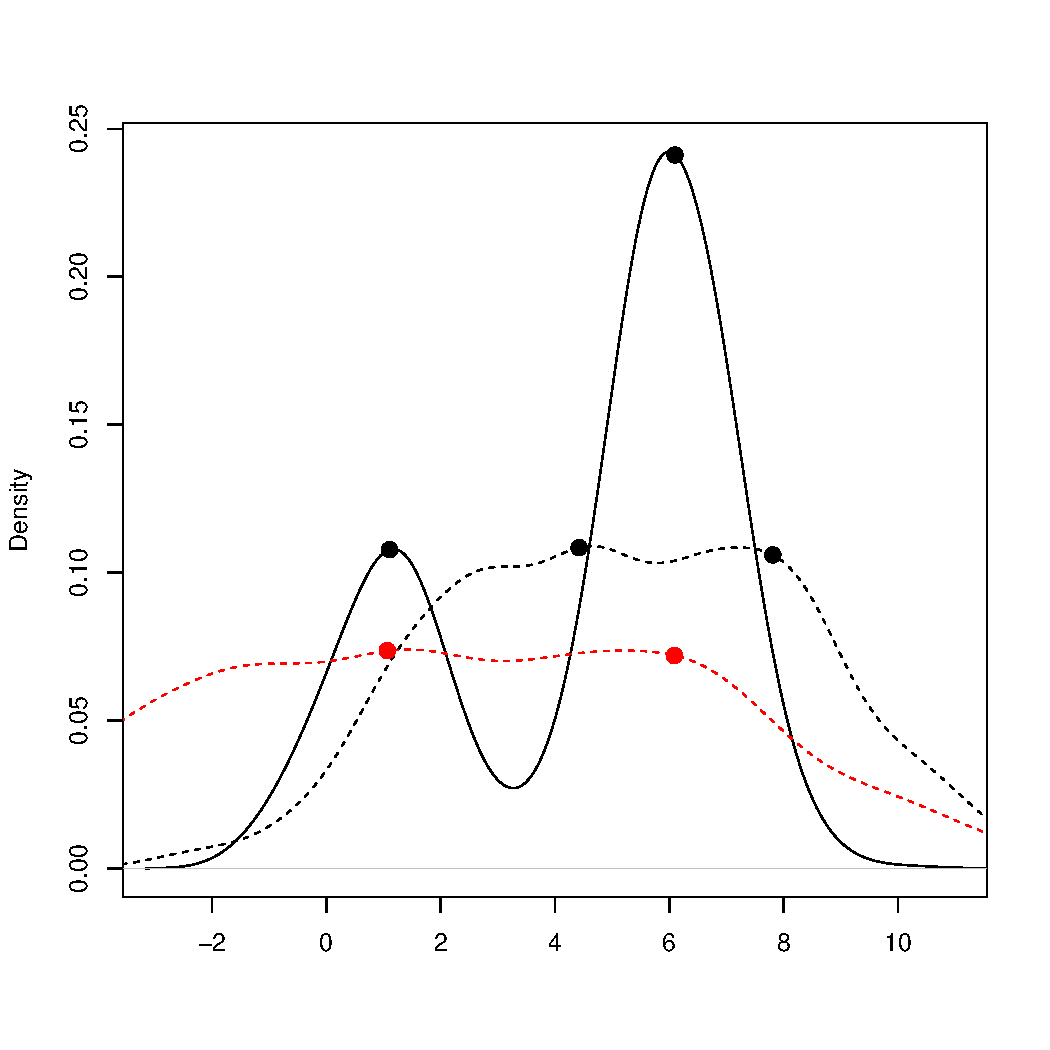
\includegraphics[scale=1]{IL2/figures/simulation-peak-align-noise.pdf}
    %\caption{  \label{figure:simulation-peak-align-noise}  In solid black line represents the density function obtained from $1000$ draws from a mixture of two normal distribution
    %with means $\mu_0=(1,6)$, standard deviations $\sigma_0=(1,1)$ and mixing proportions $\tau_0=(.3,.7)$.
    %The dashed black line represents the density function obtained from $1000$ draws from a mixture of two normal distribution
    %where $\mu_1 = 0.9 \mu_0 + 2$, standard deviations $\sigma_0=(1,1)$ and $\tau_1=(.5,.5)$.
    %The red dashed line represents the transformation using peak alignment. }
%\end{figure}
%



\section{Normalisation with controls}

The normalisation methods considered so far are data only.
However often, little is known of the data being analysed and prior knowledge can bias our analysis.
When available internal (spike-ins) or external controls, can yield a less biased normalisation technique.
Instrument variation can be detected by using a synthetic object of known and stable property which can be analysed within the sample
or independently.
In flow cytometry, fluorescent beads can be used to make intensity data comparable across days. 



\subsection{Normalisation Using Beads: Accounting for Non-Biological Variation Across Samples}


In flow cytometry, one method of normalising fluorescence intensity is to convert Mean Fluorescence Intensity (MFI)
to Molecules of Equivalent Fluorochrome (MEF) \citep{Schwartz:1996jj,Dendrou:2009bl}.
In order to apply this conversion, specially designed beads of known and (assumed) constant fluorescence defined in terms of MEF are used as a reference.
The MEF property of these beads is deemed stable whereas the MFI of the bead population is dependent on the instrument and varies over time.

The beads we use are specially manufactured so that they belong to six distinct populations of increasing MEF as shown in Table~\ref{table:fluorospheres}.
Following the bead manufacturer's guidelines, plotting the $\log_{10}(MEF)$ of these six bead populations against
the corresponding calculated $log_{10}(MFI)$ from the gated bead populations, we fit the linear regression:


\begin{equation}
    \log_{10}(\text{MEF})=\beta  \times \log_{10}(\text{MFI}) + \alpha
\label{equ:MEF}
\end{equation}

The MEF can then be obtained and is in fact a power transform of the MFI\footnote{This transform is only defined for strictly positive MFI values}:

%\[
%    MEF= 10^{\beta  \times log_{10}(MFI) + \alpha}
%]

\[
    \text{MEF}= 10^\alpha \times \text{MFI}^\beta
\]

%and so is only defined for 
%positive MFI values because $\beta$ is not an integer.

%If we add a location parameter $b$ then as expected the MEF does not scale linearly.
%\[
    %MEF= 10^\alpha \times (MFI+b)^\beta
%\]

The original MEF transform used by \citet{Dendrou:2009bl} assumes that $\beta=1$ which
gives similar results given that I found that the $\beta$ term in Equation~\ref{equ:MEF} turns out to be on average $0.96$.


In estimating the parameters $\beta$ and $\alpha$ of the linear model, only the non blank beads are used because the MEF of the blank beads is not specified by the manufacturer.
In fact extrapolating the MEF of the blank beads yields the detection threshold (Figure~\ref{figure:mef}) which we will see can be used in defining positive cell subsets.
The MEF of the blank beads is always greater than the intercept $\alpha$  which represents the log offset (the zero channel value).
%Below this threshold the intensity is meaningless as the blank beads contain by design no fluorochrome.

Typically even bead data is gated manually.
Here, in order to obtain $\beta$ and $\alpha$ parameters of the MEF transform, I will use an automatic process to gate the beads.

\begin{table} [hb]
\begin{center}
\begin{tabular} {|c c c c c c|}
\cline{1-6}
Population & FITC & RPE & REP-Cy5 & \textbf{APC} & PE-Texas Red\\
\cline{1-6}
1 & B & B & B & \textbf{B} & B \\
2 & 2,500 & 1,500 & 750 & \textbf{4,100} & 552\\
3 & 6,500 & 4,400 & 2,100 & \textbf{10,300} & 2,014\\
4 & 19,000 & 14,500 & 6900 & \textbf{25,500} & 6,975\\
5 & 55,000 & 43,800 & 22,100 & \textbf{67,300} & 20,685\\
6 & 150,000 & 131,200 & 77,100 & \textbf{139,100} & 71,888\\
\cline{1-6}
\end{tabular}
\end{center}
\caption{ \label{table:fluorospheres} FluoroSpheres from DakoCytomation. 
    The Molecules of Equivalent Fluorochromes (MEF) values for the six bead populations as provided by the manufacturer.
    B denote the blank beads which by design contain no fluorochrome.
    Of the six fluorochromes contained by each bead only APC is used in the experiment.
 }
\end{table}

\begin{figure}[hb]
    \centering
    \includegraphics[scale=0.6]{IL2RA/figures/BeadNormalisation/MEF.pdf}
    \caption{ Linear regression of bead MFI against MEF. The horizontal dash lines represent the MEF of the six bead populations.
    The red and green vertical lines define the range of memory CD25 MFI across all samples in \citet{Dendrou:2009dv}. }
    \label{figure:mef}
\end{figure}



Because all beads are known to be of identical shape and size, we expect a single cluster in the scatter channels.
Events which lie away from the main bead population are deemed to be beads clumped together or debris and so are discarded.
This can be done by fitting a bivariate normal distribution on forward and side scatter and only keeping the 95th percentile..
Once we have identified the main bead population we known that the beads belong to six populations distinguishable in the APC channel.

%We will see that these two steps are easily automated using existing tools (FlowClust on the scatter and K-Medoids on the APC channel)
%which implies that gating of bead data can be fully automated.
%Which in turn implies that channel normalisation using beads no longer needs to be a manual process.

Having gated the singlets, I subset the data and proceed to gate on the fluorescence channels to identify the six bead populations.
Since the bead population are distinguishable on all five fluorochromes (Table~\ref{table:fluorospheres}) it was first considered to use to gate on all five fluorescent channels at the same time.
However, as we are solely interested in the APC channel, it was decided better to adhere to the bead manufacter's protocol (see Fluorospheres reference manual) of only gating on the channel of interest (APC channel).
Furthermore the detectors on the flow cytometer on which the beads were run are not properly calibrated for the other fluorochromes and so the signal is noisy which adds variance to the APC signal.
%However as FlowMeans is not capable of gating on only one dimension given that the number of cluster K is known and that the bead data is quite clean, more fundamental clustering alternatives were sought.
Given that the number of clusters K is known, that the bead data is clean and the number of event is small (in the order to 10,000), we can apply the K-medoid algorithm.


\begin{figure}[ht]
%\begin{center}
    \begin{subfigure}[b]{.5\textwidth}
        \centering
        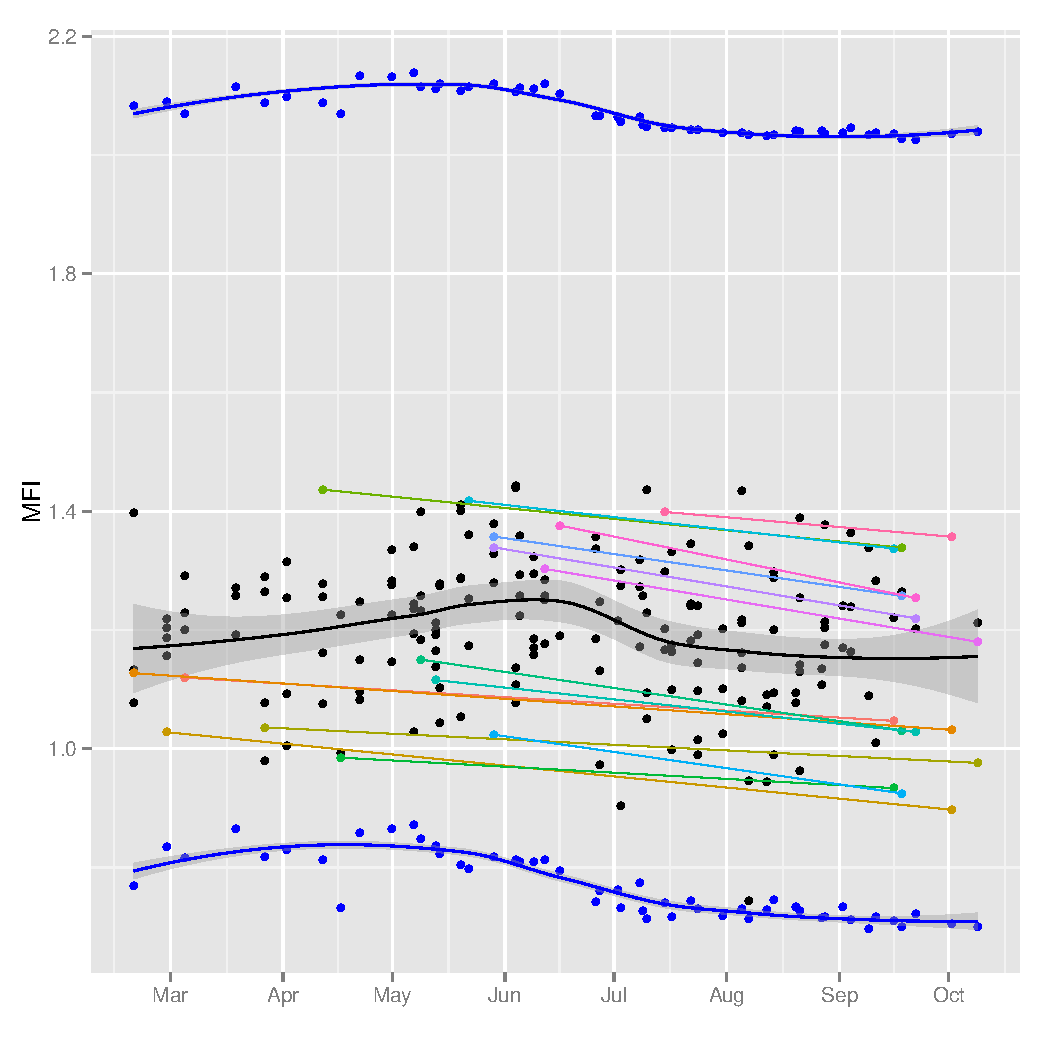
\includegraphics[scale=.5]{IL2RA/figures/CD25-MFI-time-effect-repeatability.pdf}
        \caption{Unormalised.}
    \end{subfigure}
    ~
    \begin{subfigure}[b]{.5\textwidth}
        \centering
        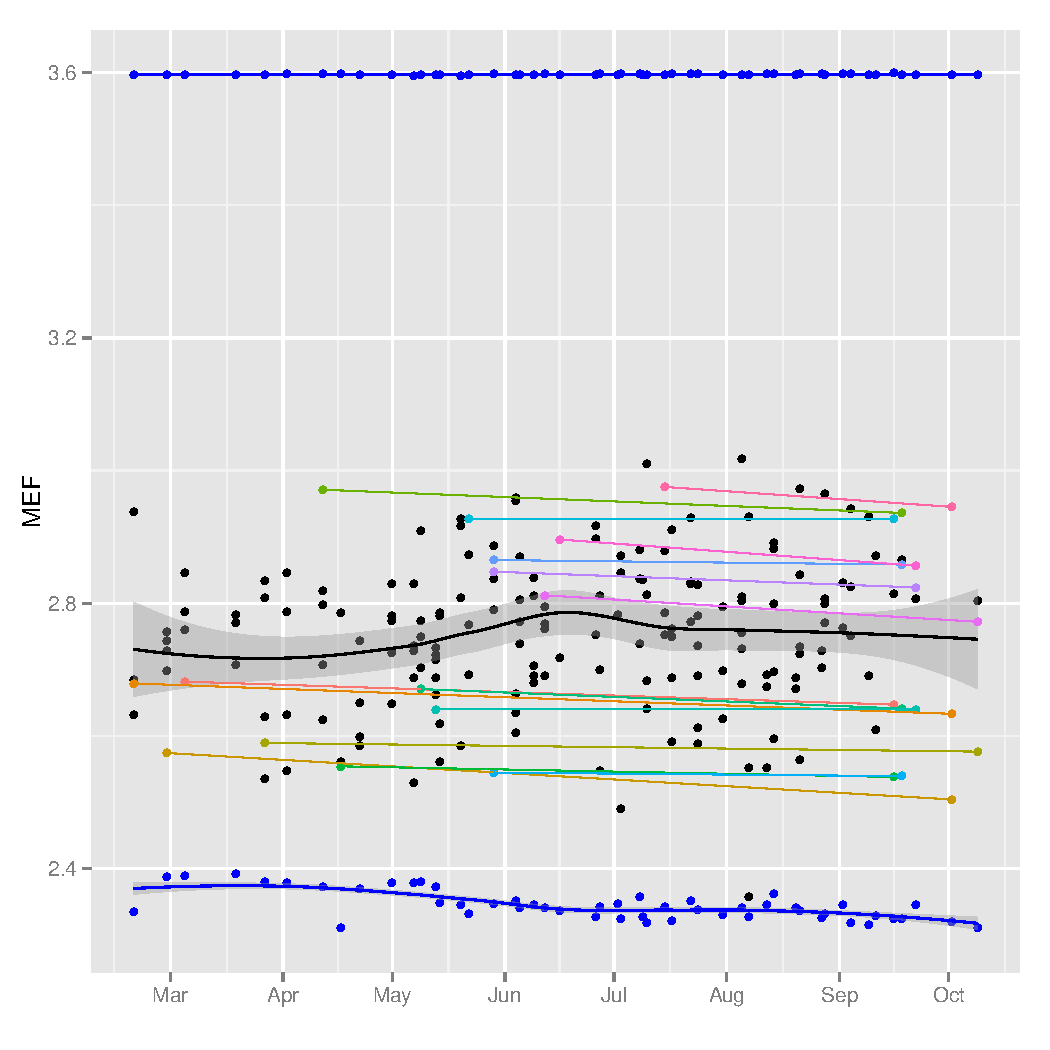
\includegraphics[scale=.5]{IL2RA/figures/CD25-MFI-time-effect-beads-normalised.pdf}
        \caption{Normalised}
    \end{subfigure}
    ~
    \begin{subfigure}[b]{.5\textwidth}
        \centering
        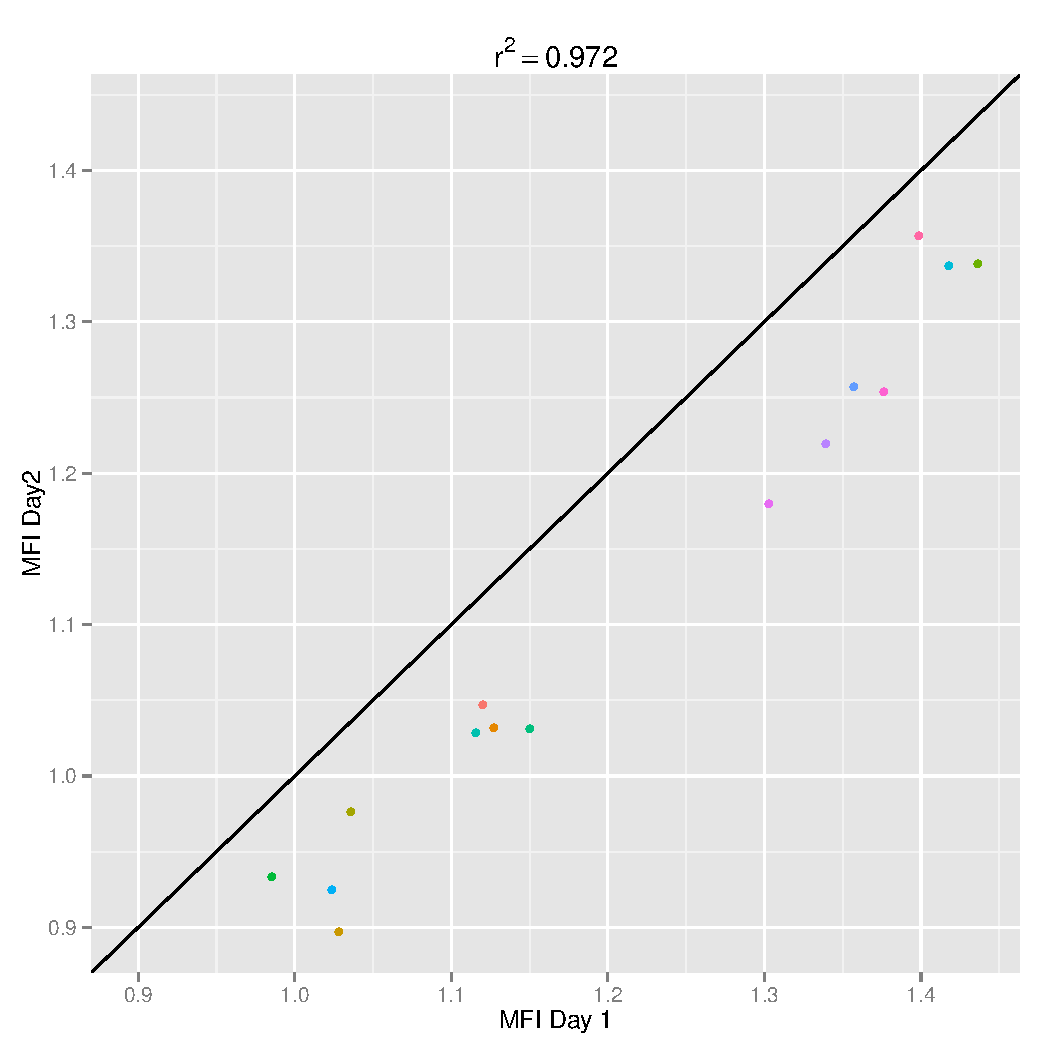
\includegraphics[scale=.75]{IL2RA/figures/CD25-MFI-repeatability.pdf}
        \caption{Unormalised: $R^2=0.629$}
    \end{subfigure}
    ~
    \begin{subfigure}[b]{.5\textwidth}
        \centering
        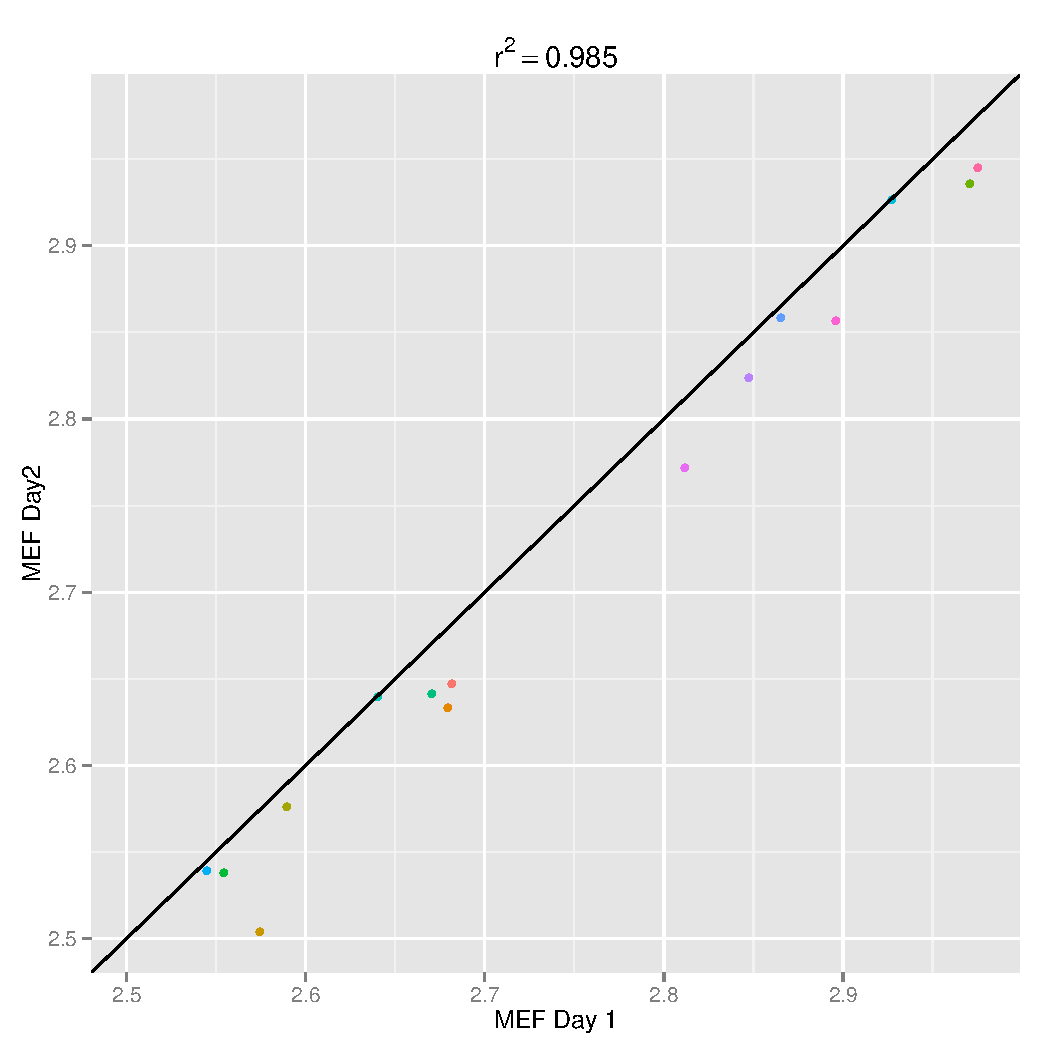
\includegraphics[scale=.75]{IL2RA/figures/CD25-MFI-beads-normalised.pdf}
        \caption{Normalised: $R^2=0.937$}
    \end{subfigure}
%\end{center}
    \caption{ \label{figure:CD25-MFI-beads-normalised.pdf}
\textbf{Bead normalisation partially corrects for long term time effect in CD25 MFI of the memory cell population.}
In \textbf{(a)} and \textbf{(b)}, the blue points represent the MFIs of the bead populations, in black the MFIs of the memory cell populations.
A loess is fitted to the MFIs of the beads and memory cells.
The points joined by lines are MFIs from recalled individuals.
The normalisation step involves aligning the peaks of the two bead populations across days to the overall mean of each of the populations (the dashed blue).
The normalisation improves the repeatability of the MFI in recalled individuals from $R^2=0.629$ \textbf{(c)} to $R^2=0.937$ \textbf{(d)}.
}
\end{figure}


\section{Normalisation of pSTAT5}

In Figure~\ref{figure:channels-doses}, considering the density functions across all channels in resting lymphocytes compared to ones stimulated at the highest dose,
there seems to be no need for normalisation since the peaks in the density plots align well.
%normalisation is not required to account for dose effects.
Considering unstimulated lymphocytes across days however, Figure~\ref{figure:channels-days} suggests that there is need for normalisation since the distributions do not always align well.
See for example individual b for marker CD45RA.

\begin{figure}[h]
    \centering
    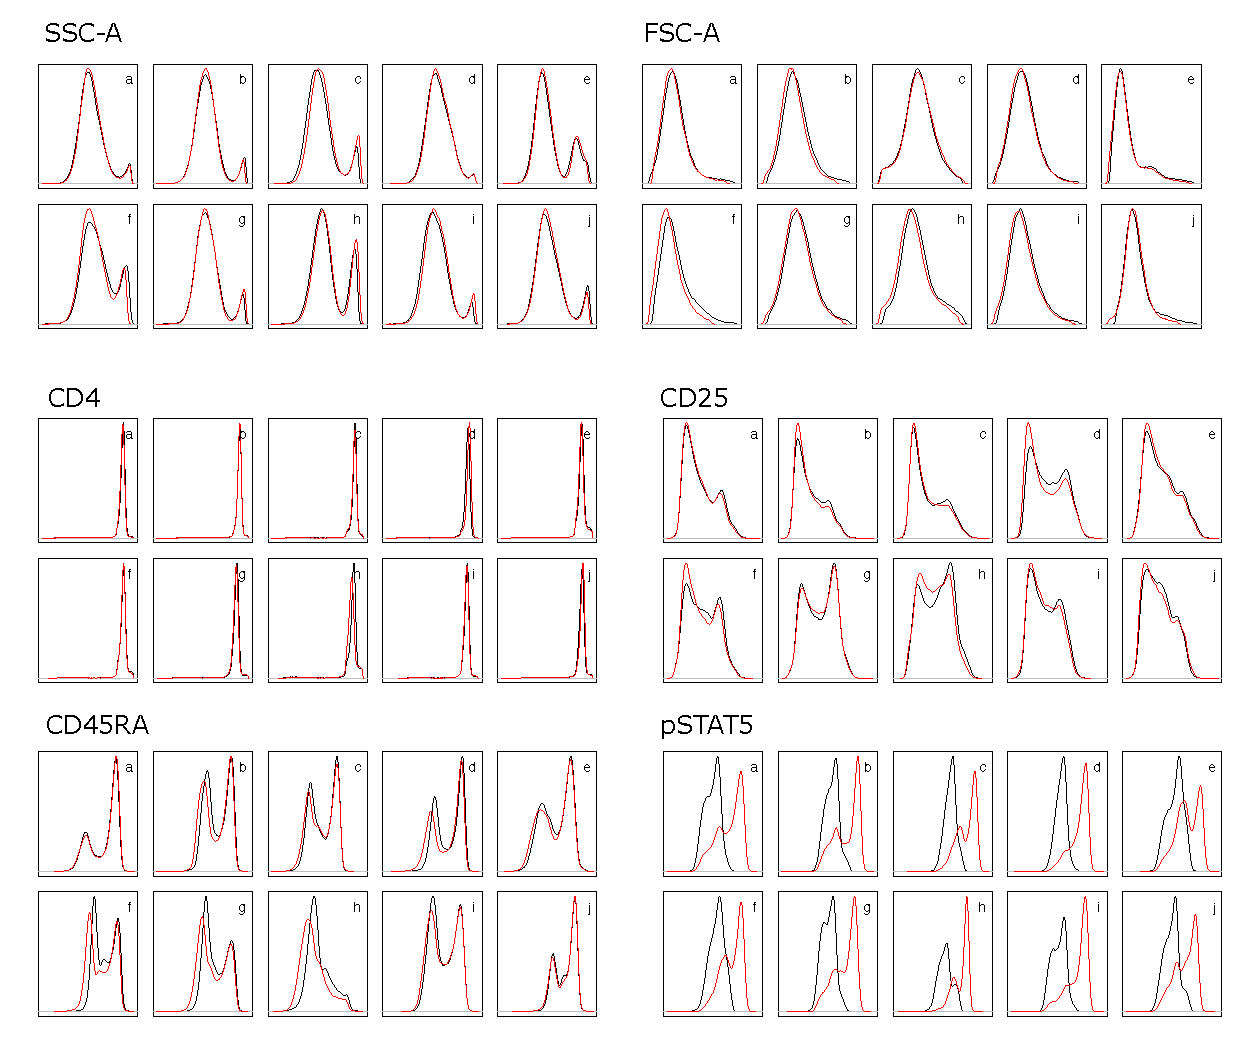
\includegraphics[scale=.75]{IL2/figures/channels-doses.pdf}
    \caption{  \label{figure:channels-doses} 
    In CD4 lymphocytes on same day different doses in 10 individuals (a, b, c, d, e, f, g, h, i, j).
  Black resting doses, in red 1000UL stimulation. As expected as a result of the stimulation, the peak of the pSTAT5 distribution shifts. }
\end{figure}


\begin{figure}[h]
    \centering
    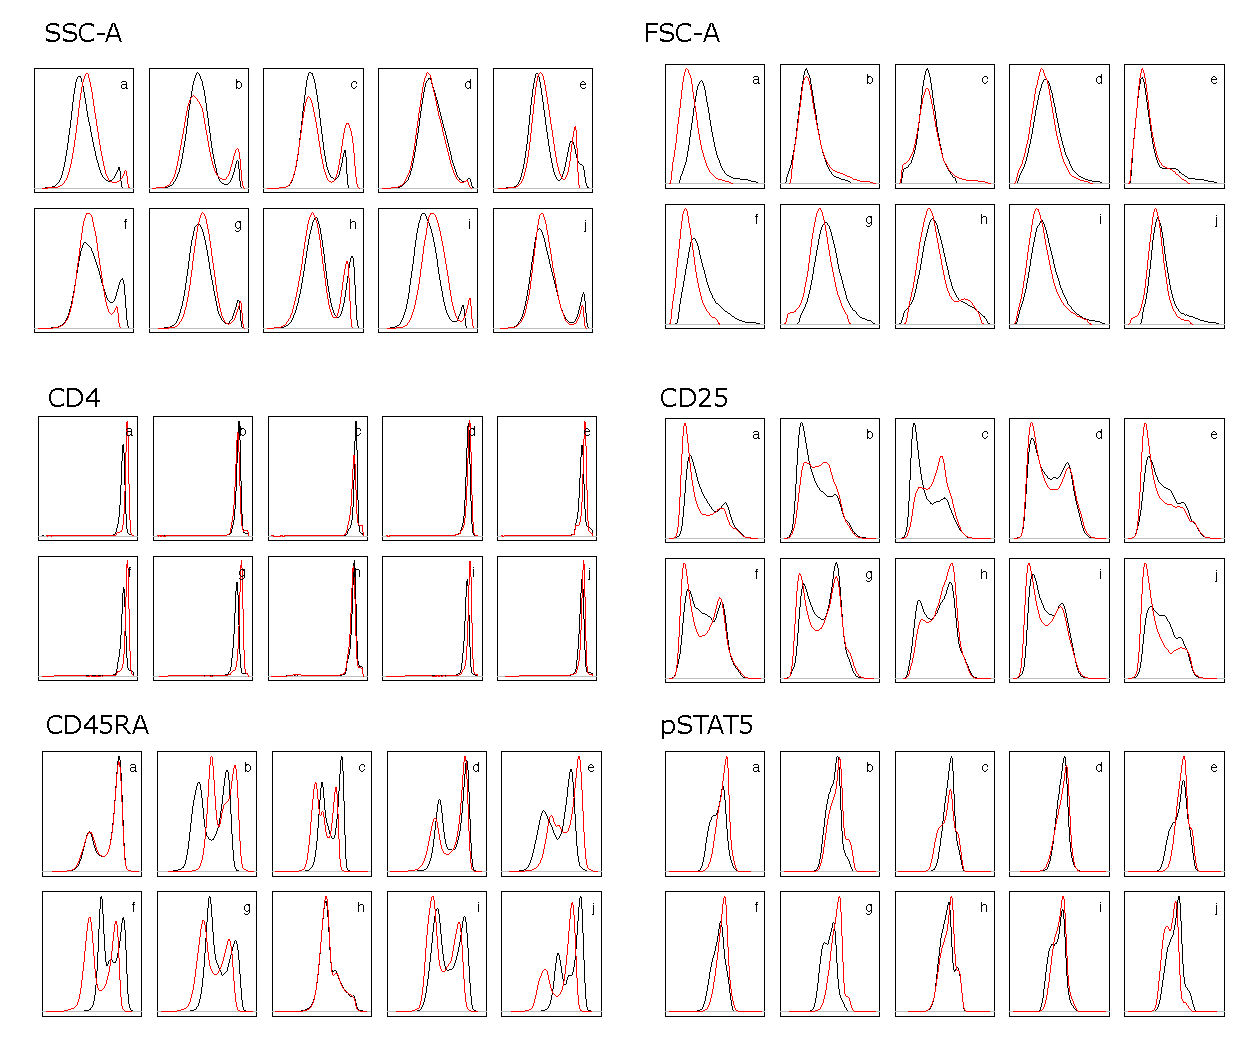
\includegraphics[scale=.75]{IL2/figures/channels-days.pdf}
    \caption{  \label{figure:channels-days} 
    In resting CD4 lymphocytes for each of the 10 individuals (a, b, c, d, e, f, g, h, i, j), black the first day and in red the second day.
    The distributions no longer appear to align as well. This suggests there might be need for normalisation to realign the peaks.}
\end{figure}


If we expect that the core cell populations should exist in all samples but that their locations and their
proportions may vary across days and \emph{IL-2} dose, 
a normalisation approach is to align the location of the population across doses per day while allowing for the relative proportion of the populations to vary.

\begin{figure}[h]
    \centering
    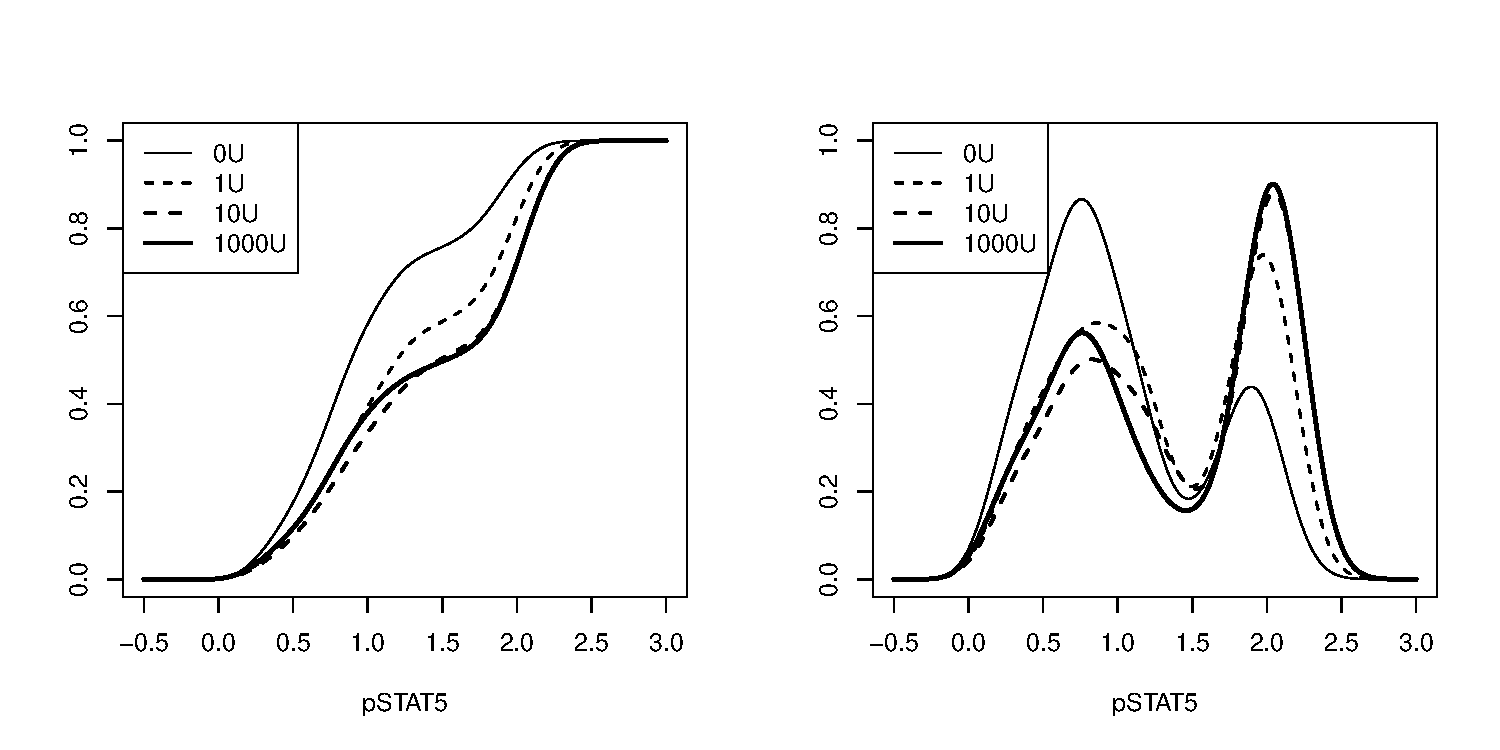
\includegraphics[scale=.5]{IL2/figures/ungated-dose-effect.pdf}
    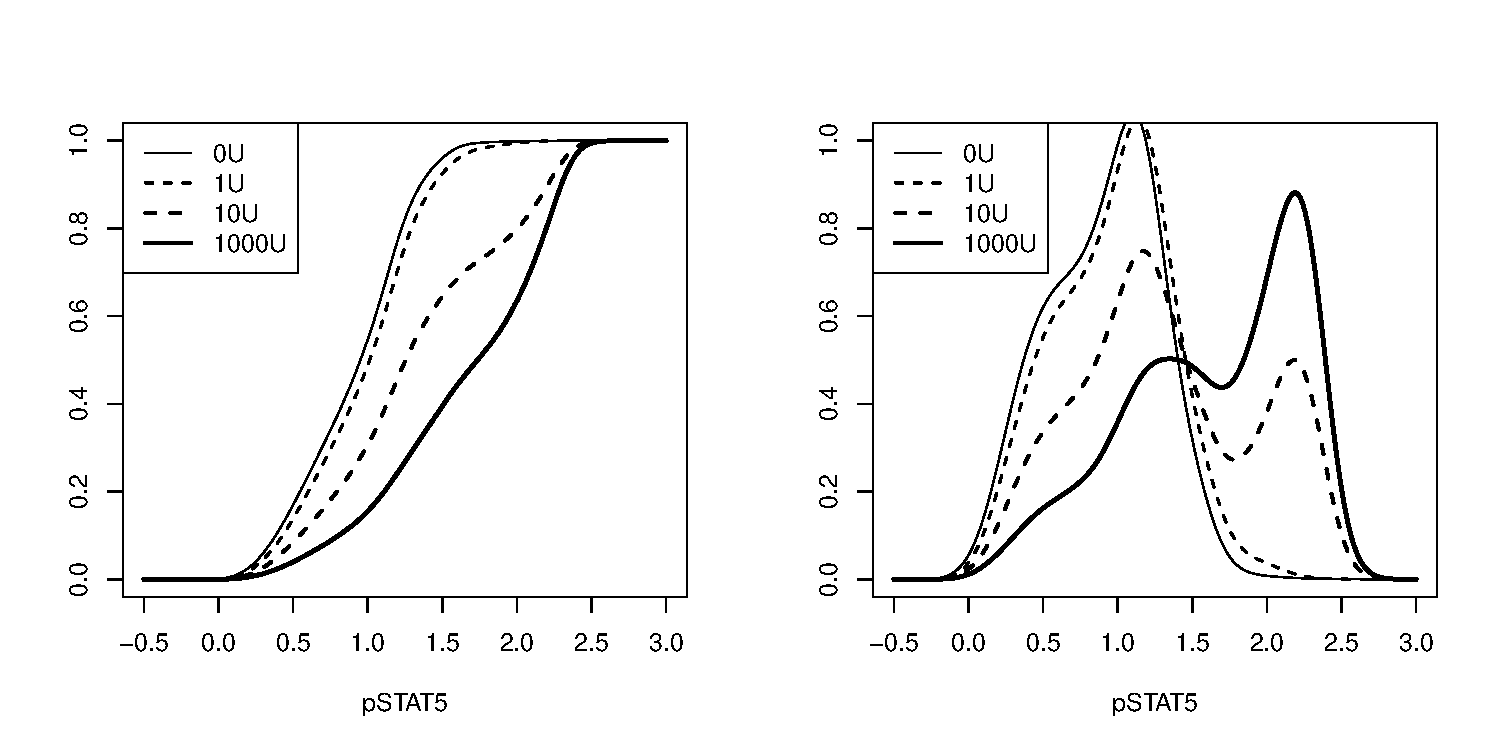
\includegraphics[scale=.5]{IL2/figures/lymph-dose-effect.pdf}
    \caption{  \label{figure:dose-effect}
        On the left the cumulative density function obtained from individual a on day 1 across 4 increasing doses.
        On the right the density function.
        The top two figures are from the ungated sample.
        The bottom two figures are from a CD4 range gate.
        We observe that in the unstimulated sample the distribution is already bimodal 
        and that upon stimulation the location of the peaks does not change much but that the height changes greatly.
        Contrary to the ungated data, the pSTAT5 distribution in the CD4 gated sample now appears unimodal when resting or stimulated
        at the lowest 1U dose.  At the higher doses we start seeing a bimodal distribution.
        In the ungated sample, the location of the activation peak seems to align somewhat with that of the activation peak.  }
\end{figure}

Another method is to not concern ourselves with aligning the cell populations but instead to focus on the reproducibility of the response in terms of relative shift in the pSTAT5 distribution across days in various cell populations.
The idea being that unstimulated sample should yield the baseline on that day.

The relative shift in the pSTAT5 distribution between resting and stimulated can be measured by computing the area between the cumulative density functions of the unstimulated and stimulated samples.

In Figure~\ref{figure:dose-effect} we observe that the dose effect is very different in the ungated than in the CD4 gated subset (lymphocytes) which represent around $10\%$ of
the whole sample.
The lowest 1U dose seems to have a much more stronger relative effect in the whole sample than in the lymphocyte subset which suggest that there sizeable amount of cells in the ungated
data which are much more sensitive to low doses of IL-2 than the lymphocytes.
However the relative difference in response between 10U and 1000U seems much more important in lymphocytes than in the whole sample
Also since the resting sample sample display a shoulder in resting state it seems that lymphocytes even in a resting state are a mixture of resting and semi-activated lymphocytes.


In the manual analysis conducted by Tony Cutler, he found that he could identify individuals which were low or high responders.
This leads us to hypothesise that within one individual the response to \emph{IL-2} on day 1 should be comparable to the response to \emph{IL-2} on day 2.

%One method we have tried is based on the assumption is that in the ungated data, the bottom and top percentile of the pSTAT5 distribution do not respond to \emph{IL-2} and so can be used as reference points.  This is effectively a quantile normalisation method aligning the bottom and top percentile across doses.

%However we found that this normalisation method d is not true in CD4+ lymphocyte gated data.

\section{Discussion}

%Sometimes it is better not to normalise and normalisation may hide the true biological effect.

Certain normalisation methods make assumptions about the shape of the data.
The actual choice of normalisation depends on the characteristics of the data we wish to compare.

We have only considered the univariate density function here but identification can be extended to the multivariate case.

Next let's consider normalisation of multivariate distributions.  
The purpose of principal component correction is to remove unwanted correlation between samples.

When applying a linear transform to multivariate data the correlation between the dimensions is preserved since the multiplicative factors cancel out.
However the covariance changes.
Care must be taken when applying a non-linear transform.  

Normalisation is effectively analogous to meta-clustering since we are attempting to match cell populations across samples.  
Normalisation facilitates matching clusters across datasets but in doing can remove meaningful biological variation.  


A less biased approach is to allow for different cluster location and shapes across datasets and instead incorporate the clustering in some sort of hierarchical framework.  
Normalisation or meta-clustering is a necessary step when data is pooled across studies.



\chapter{\label{appendix:clustering}Clustering}

\section{K-means and K-medoids}

Due to implementation simplicity and speed, the K-means algorithm is possibly the most well established and widely used clustering algorithm.
As I will show, the algorithm can been reparameterised and extended in many interesting ways to make it more flexible.
The objective function of K-means is to try to minimise the overall sum of within-cluster sum of squares.

\[
    \sum_{k=1}^{K} \sum_{\mathbf x_i \in S_k} ( \mathbf x_i - \boldsymbol\mu_k )^2 ; \quad \boldsymbol\mu_k=\text{E}(x_i| x_i \in S_k)
\]


The algorithm starts by picking K random points which are the initial guess as to where the cluster means lie.
Then for each iteration:
\begin{itemise}
    \item Each point $x_i$ is assigned to the cluster $S_k$ of the closest current cluster mean $\mu_k$.
    \item Based on this new cluster assignment, the new cluster mean of each cluster is computed.
\end{itemise}
The algorithm terminates when no cluster mean changes.

\vspace{1em}
\noindent

K-means is extremely fast since it only requires $N \times K$ operations at each iteration.
However, it is sensitive to starting conditions and skewed data because of its reliance on the mean function.
These shortcomings are addressed by a related but slower algorithm: K-medoids.
Instead of using the cluster means, K-medoids updates the cluster medoids.
The medoid is defined as the point of the cluster which minimises the overall distance
to all other points belonging to that cluster.
The objective function of K-medoids is therefore:

\[
    \sum_{k=1}^{K} \sum_{\mathbf x_i \in S_k} ( \mathbf x_i - \boldsymbol M_k )^2 ; \quad \boldsymbol M_k=\text{Medoid}(x_i| x_i \in S_k)
\]

Since the medoids can only be points of the dataset, the complete distance matrix need only be calculated once at the onset.
The algorithm starts by picking K starting points which belong to the set of data points.
These represent the initial guess as to where the cluster medoids lie.
Then for each iteration:
\begin{itemise}
    \item Each point $x_i$ is assigned to the cluster $S_k$ of the current closest cluster medoid $M_k$.
    \item Based on this new cluster assignment, the new cluster medoid of each cluster is selected.
\end{itemise}
The algorithm terminates when no cluster medoid changes.
The algorithm is reasonably fast but can be slower for larger datasets due to the first step of calculating the complete distance matrix.
For sufficiently large $N$, the size of the distance matrix may be prohibitive and too large for memory.
Therefore this version of the algorithm may not scale to large $N$ as well as K-means. 
%There exists an implementation in R which works on subsets of the data and combines the results: clara



\section{Adding parameters: generalising K-means to Gaussian Mixture Models}

As discussed, the objective function of K-means is to try to minimise the overall sum of within-cluster sum of squares:
\[
    \sum_{k=1}^{K} \sum_{\mathbf x_i \in S_k} ( \mathbf x_i - \boldsymbol\mu_k )^2 ; \quad \boldsymbol\mu_k=\text{E}(x_i| x_i \in S_k)
\]

One shortcoming of K-means is that it does not account for the uncertainty in classifiying points.
Each point is the responsibility of a single cluster.
An alternative notation which helps parameterise the problem is to define the $N$ by $K$ matrix $\mathbf Z$ of responsibilities:

\[
\mathbf Z =
 \begin{pmatrix}
  1 & 0 & \cdots & 0 \\
  0 & 0 & \cdots & 1 \\
  \vdots  & \vdots  & \ddots & \vdots  \\
  0 & 1 & \cdots & 0
 \end{pmatrix}
\]

If the ith point of the dataset belongs to to cluster k then $Z_{i,k}=1$, otherwise $Z_{i,k}=0$.
This implies that every row of $Z$ sums to 1 and that the columns sum to the number of points within each cluster.
We can now rewrite the overall sum of within-cluster sum of squares as:

\[
  \sum_{i=1}^N \sum_{k=1}^{K} ( x_i z_{ik} - \operatorname{E}(x_i z_{ik}) )^2 
\]

Further, if each cluster is scaled by its size then this can by rewritten in the one-dimensional case as:


\[
  \sum_{k=1}^{K} \operatorname{VAR}(\mathbf Z_k \mathbf X)
\]


If we allow probabilistic assignment of data points to clusters $\mathbf Z$ matrix, while maintaining the constraint that each rows sums to 1,
then the matrix may take the form:


\[
\mathbf Z =
 \begin{pmatrix}
  0.3 & 0.1 & \cdots & 0.4 \\
  0.5 & 0.25 & \cdots & 0.1 \\
  \vdots  & \vdots  & \ddots & \vdots  \\
  0.1 & 0.8 & \cdots & 0.05
 \end{pmatrix}
\]

This extension can be considered a fuzzy variant of K-means.

If we use the Mahalanobis distance, which 
takes the variance of the clusters into account in the distance computation,
then we obtain the following univariate mixture of Gaussian distributions:
\[
\sum_{k=1}^K\tau_k \frac{1}{\sigma_k\sqrt{2\pi}} e^{ -\frac{(x_i-\mu_k)^2}{2\sigma_k^2} }; \quad \sum_{k=1}^K\tau_k = 1
\]



Then the above can be rewritten as:


\[
  \sum_{k=1}^K \operatorname{E}(\mathbf Z_k) \frac{1}{\sqrt{2\pi \operatorname{VAR} (\mathbf Z_k \mathbf x_i)} } e^{ -\frac{(\mathbf x_i- \operatorname{E}(\mathbf Z_k \mathbf x_i))^2}{2\operatorname{VAR}(\mathbf Z_k \mathbf x_i)} }
\]



Multivariate mixture of Gaussian distributions:
\[
\sum_{k=1}^K\tau_k \frac{1}{\sqrt{(2\pi)^2|\boldsymbol\Sigma_k|}}
e^{-\frac{1}{2}({\mathbf x_i}-{\boldsymbol\mu_k})^T{\boldsymbol\Sigma_k}^{-1}({\mathbf x_i}-{\boldsymbol\mu_k})
}; \quad \sum_{k=1}^K\tau_k = 1
\]


\section{Parameter constraints: regularisation} 
%\section{Clustering with priors}

Algorithms proceed in an iterative fashion to explore the parameter space with the objective of finding a global optimum of the
least-squares or likelihood function.
The stopping criterion is reached upon convergence of the objective function or equivalently of the parameter updates.
However local optimums of the objective function can also lead to convergence.
There are also regions of the parameter space which need to be avoided.
For example, the likelihood function can also be made arbitrarily large if the variance of a cluster is allowed to shrink to zero.

%One pitfall of these methods is that the objective landscape may contain many local minimum or maximums 
To safeguard from these situations,
some guidance can be provided by picking sensible starting conditions or by fixing hard boundaries on the parameter space.
Another softer approach is to weight parameter updates with a distribution.
This approach is also called regularisation.
Regularisation can be achieved using a prior probability density function on the parameters.

Formally, let $X$ be the data and $\theta$ be the parameters of the random distribution that generated $X$, then Bayes theorem tells us that:

\[
P(\theta|X) = \frac{P(X|\theta) P(\theta)}{P(X)}
\]

\noindent

where $P(\theta)$ is the prior, $P(X)$ is the evidence, $P(X|\theta)$ the marginal likelihood over the data and $P(\theta|X)$ is posterior.
Given the probability density function $P$, the objective is to find $\theta$ which maximises the posterior and so the likelihood:

\[
\mathcal{L}(\theta |X) = P(X | \theta)
\]

Given $\theta$, the likelihood $P(X|\theta) \propto $  density function:

\[
\mathcal{L}(\theta |X) = \prod_{i=1}^N p(x_i|\theta).
\]

Since a product of small numbers is numerically unstable, the logarithm of the likelihood is preferred:


\[
\ln \mathcal{L}(\theta |X) = \sum_{i=1}^N \ln p(x_i|\theta).
\]



%The entries in the matrix $Z$ contain the posterior probability of $X_i$ belonging to population $k$:
%\[
%P(X_i \in k | n) = \frac{\pi_k d_k(X_i)} {\sum_{p=1}^{P} \pi_p d_p(X_i)}
%\]
%\noindent
%$\sum_{p=1}^{P} \pi_p d_p(X_n)$ represents the density as estimated by fitting the mixture model.
%

\section{Hard or soft?}

The time of convergence of the parameters depends on the softness of the method.
For example soft k-means takes longer to converge than hard k-means since the matrix of posterior probabilities is updated in small steps.
%Generally large updates in parameter estimates tend to converge faster but to less optimal solutions.
%In gradient descent, the step size is inversely proportional to the gradient, so that flat regions of the parameter space are explored faster.
%Small updates to the objective function translate to small parameter updates.

Another issue with soft clustering approaches is if the number of components is large and the method is too soft, than assignment cannot be achieved with
any degree of certainty (low max posterior probability).
This is usually an indication that the data is too noisy.



% example of kmeans fail on skewed data
%\begin{figure}[h]
    %\centering
    %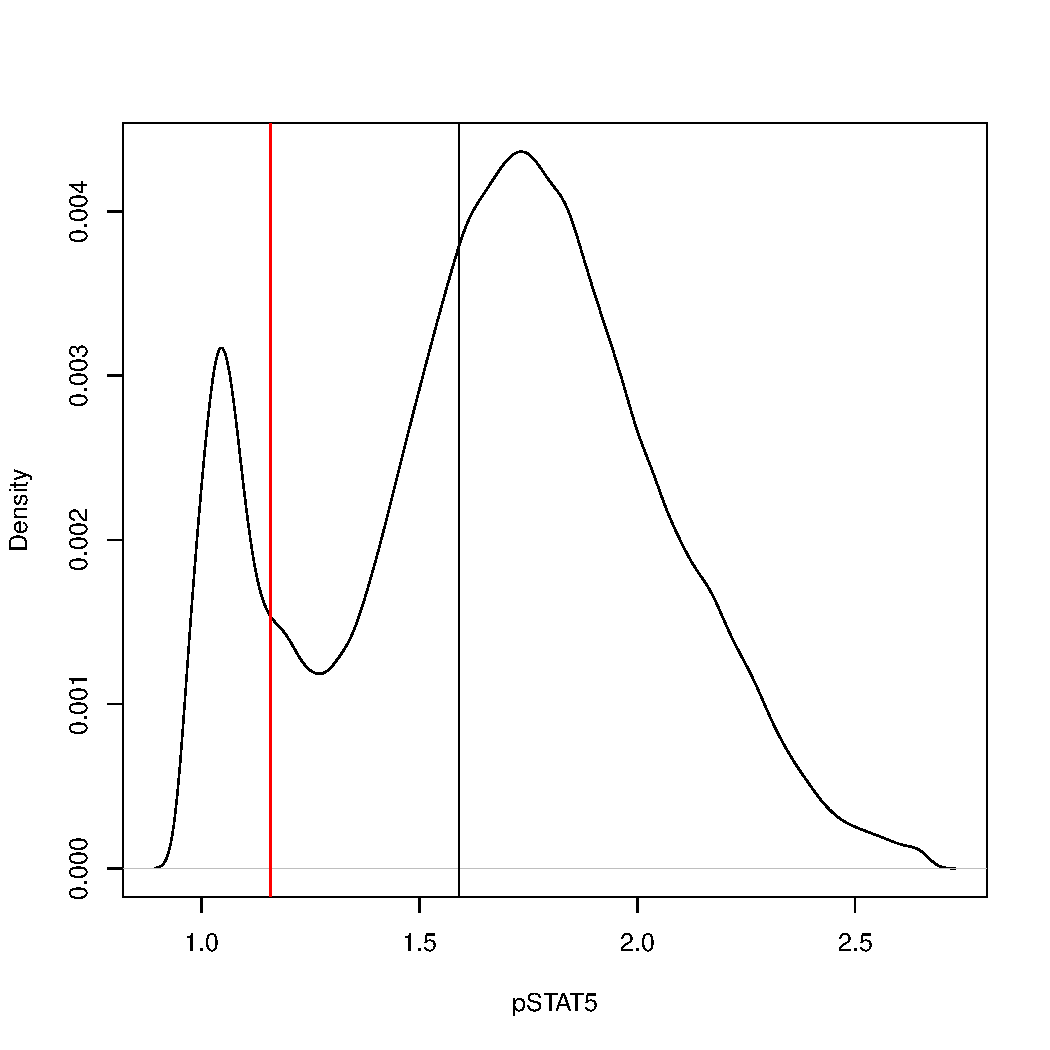
\includegraphics[scale=.5]{IL2/figures/kmeans-fail.pdf}
    %\mycaption{figure:kmeans-fail.pdf}
    %{Kmeans can fail to partition clusters when the clusters are of very uneven size (black vertical line).}
    %{
      %Fitting a mixture model allows for different cluster variance and so provides a better partitioning of the clusters.
    %}
%\end{figure}
%


\chapter{\label{appendix:flowsorting}{Flow markers}}

\paragraph{CD3} Found on all T cells.

\paragraph{CD8} Marker of cytotoxic T cells or killer cells.

\paragraph{CD4} Found on a subset of T lymphocytes and helper cells.
%A response orchestrator.

\paragraph{CD31} Largely present on naive CD4 T cells.
Lost on maturation of naive cell after leaving the thymus.
%Recent thymic emigrants.

\paragraph{CD45RA} Isoform of CD45 lost on activation of naive CD4\positive and CD8\positive T cells.
Can be used to distinguish CD45RA high naive cells from CD45RA low memory cells.

\paragraph{CD127}
The alpha chain of the IL-7 receptor.
The IL-7 receptor is expressed on various cell types, including naive and memory T cells,
and usually expressed at higher levels on T effector and regulatory T cells.

\paragraph{CD25}
Better known as the \protein{IL2RA}, the alpha chain of the heterotrimeric IL-2 receptor.
High affinity binding of IL-2 requires all three chains of the receptor.

\paragraph{CD122}
The beta chain of the IL-2 receptor, also known as IL2RB.

\paragraph{CD132}
The gamma chain of the IL-2 receptor, also known as IL2RG.

\paragraph{CD56}
NK cell marker.


\paragraph{CD19}
Found on the surface of B-cells.
Expressed on follicular dendritic cells and B cells.
Also a lineage marker which is lost on maturation to plasma cells.

\paragraph{CD69}
A protein induced by the activation of T lymphocytes and Natural Killer cells.
Involved in lymphocyte proliferation and functions as a signal-transmitting receptor in lymphocytes.

 
%\chapter{ Normalisation of fluorescence intensity using beads }
%%\subsection{Normalisation Using Beads: Accounting for Non-Biological Variation Across Samples}

The objective of flow cytometry is to capture variation in the biological sample not variation linked to the instrument or to other experimental factors.
Normalisation is the process of factoring out non-biological for sensible comparison fo samples analysed at different times or on different instruments.
In flow cytometry, one method of normalising fluorescence intensity is to convert Mean Fluorescence Intensity (MFI)
to Molecules of Equivalent Fluorochrome (MEF) \citep{Schwartz:1996jj,Dendrou:2009bl}.
In order to apply this conversion, specially designed beads of known and (assumed) constant fluorescence defined in terms of MEF are used as a reference.
The MEF property of these beads is deemed stable whereas the MFI of the bead population is dependent on the instrument and varies over time.

In our case, the beads used are specially manufactured so that they belong to six distinct populations of increasing MEF as shown in Table~\ref{table:fluorospheres}.
Following the bead manufacturer's guidelines, plotting the $\log_{10}(MEF)$ of these six bead populations against
the corresponding calculated $log_{10}(MFI)$ from the gated bead populations, we fit the linear regression:

\begin{equation}
    \log_{10}(\text{MEF})=\beta  \times \log_{10}(\text{MFI}) + \alpha
\label{equ:MEF}
\end{equation}

The MEF can then be obtained and is in fact a power transform of the MFI\footnote{This transform is only defined for strictly positive MFI values}:

%\[
%    MEF= 10^{\beta  \times log_{10}(MFI) + \alpha}
%]

\[
    \text{MEF}= 10^\alpha \times \text{MFI}^\beta
\]

%and so is only defined for 
%positive MFI values because $\beta$ is not an integer.

%If we add a location parameter $b$ then as expected the MEF does not scale linearly.
%\[
    %MEF= 10^\alpha \times (MFI+b)^\beta
%\]

The original MEF transform used by \citet{Dendrou:2009bl} assumes that $\beta=1$ which
gives similar results given that I found that the $\beta$ term in Equation~\ref{equ:MEF} turns out to be on average $0.96$.


In estimating the parameters $\beta$ and $\alpha$ of the linear model, only the non blank beads are used because the MEF of the blank beads is not specified by the manufacturer.
In fact extrapolating the MEF of the blank beads yields the detection threshold (Figure~\ref{figure:mef}) which we will see can be used in defining positive cell subsets.
The MEF of the blank beads is always greater than the intercept $\alpha$  which represents the log offset (the zero channel value).
%Below this threshold the intensity is meaningless as the blank beads contain by design no fluorochrome.

Typically even bead data is gated manually.
Here, in order to obtain $\beta$ and $\alpha$ parameters of the MEF transform, I will use an automatic process to gate the beads.

\begin{table} [hb]
\begin{center}
\begin{tabular} {|c c c c c c|}
\cline{1-6}
Population & FITC & RPE & REP-Cy5 & \textbf{APC} & PE-Texas Red\\
\cline{1-6}
1 & B & B & B & \textbf{B} & B \\
2 & 2,500 & 1,500 & 750 & \textbf{4,100} & 552\\
3 & 6,500 & 4,400 & 2,100 & \textbf{10,300} & 2,014\\
4 & 19,000 & 14,500 & 6900 & \textbf{25,500} & 6,975\\
5 & 55,000 & 43,800 & 22,100 & \textbf{67,300} & 20,685\\
6 & 150,000 & 131,200 & 77,100 & \textbf{139,100} & 71,888\\
\cline{1-6}
\end{tabular}
\end{center}
\caption{ \label{table:fluorospheres} FluoroSpheres from DakoCytomation. 
    The Molecules of Equivalent Fluorochromes (MEF) values for the six bead populations as provided by the manufacturer.
    B denote the blank beads which by design contain no fluorochrome.
    Of the six fluorochromes contained by each bead only APC is used in the experiment.
 }
\end{table}

\begin{figure}[hb]
    \centering
    \includegraphics[scale=0.6]{IL2RA/figures/BeadNormalisation/MEF.pdf}
    \caption{ Linear regression of bead MFI against MEF. The horizontal dash lines represent the MEF of the six bead populations.
    The red and green vertical lines define the range of memory CD25 MFI across all samples in \citet{Dendrou:2009dv}. }
    \label{figure:mef}
\end{figure}



Because all beads are known to be of identical shape and size, we expect a single cluster in the scatter channels.
Events which lie away from the main bead population are deemed to be beads clumped together or debris and so are discarded.
Once we have identified the main bead population we known that the beads belong to six populations distinguishable in the APC channel.

%We will see that these two steps are easily automated using existing tools (FlowClust on the scatter and K-Medoids on the APC channel)
%which implies that gating of bead data can be fully automated.
%Which in turn implies that channel normalisation using beads no longer needs to be a manual process.

\subsection{Bivariate Gating on Forward and Side Scatter}

%% Gating
% Scatter plots
\begin{figure}[ht]
%\begin{center}
    \begin{subfigure}[b]{.5\textwidth}
        \centering
        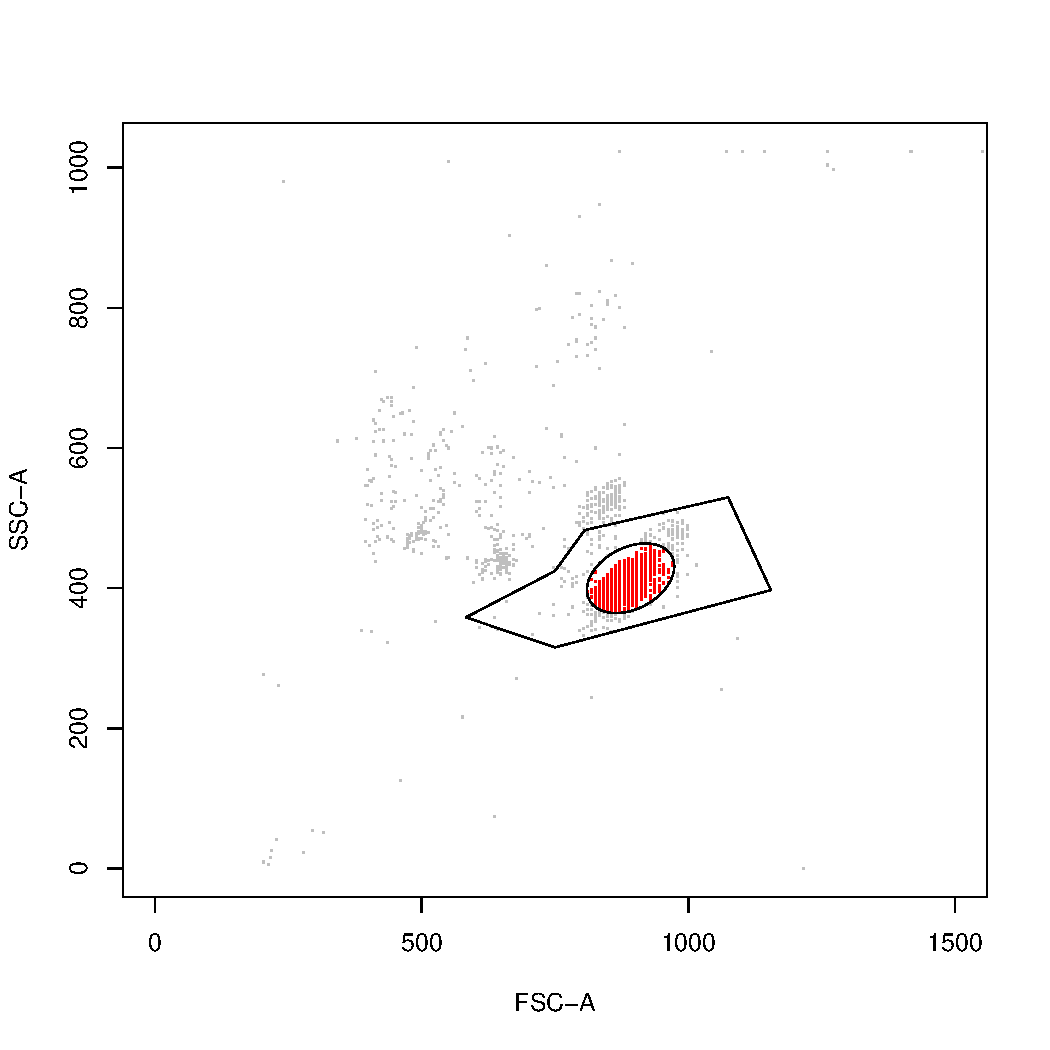
\includegraphics[scale=.5]{IL2RA/figures/Beads/manual-flowclust-scatter-gate-cad57.pdf} 
        \caption{Manual and FlowClust gating on scatter.}
    \end{subfigure}
    ~
    \begin{subfigure}[b]{.5\textwidth}
        \centering
        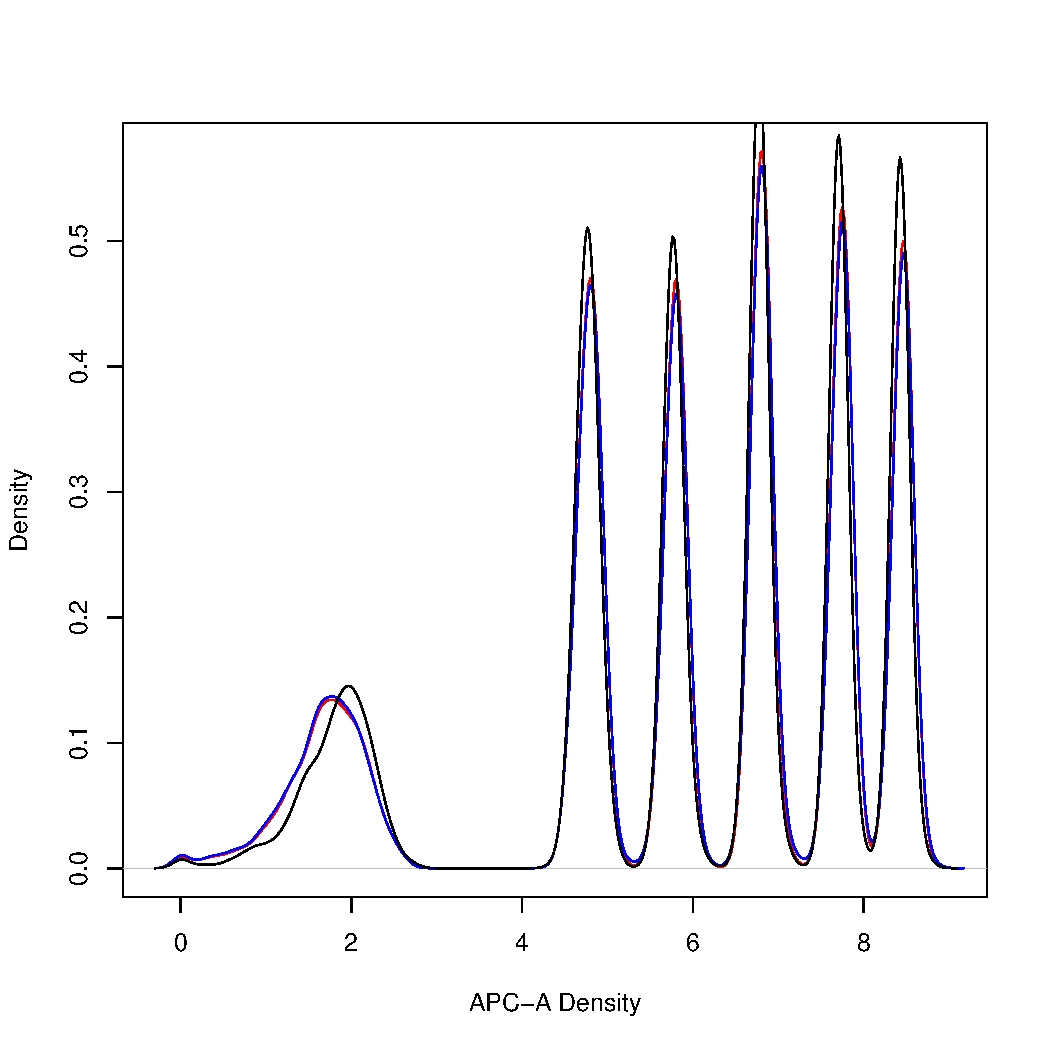
\includegraphics[scale=.5]{IL2RA/figures/Beads/manual-flowclust-apc-cad57.pdf} 
        \caption{density of $log$ APC after applying scatter gate.}
    \end{subfigure}
%\end{center}
\caption{ \label{figure:bead-gate}
  In Figure a), the gate applied by FlowClust (in red) is a subset of the gate applied through manual gating (in blue).
In Figure b) we notice that the effect of the scatter gating on the APC channel is to reduce the intensity of the first peak (the blank beads) and slightly increase the intensity of the other peaks.
Overall both manual and FlowClust gating seem to yield very similar distributions. }
\end{figure}



I first gated on both the forward and side scatter using \texttt{FlowClust} \citep{Lo:2008it}
to distinguish single beads from groups of beads which might go through the flow cytometer clumped together (Figure~\ref{figure:bead-gate}).
FlowClust proceeds by doing a Box-Cox transform to normalise the data, then fits a mixture of Student t-distributions
using the EM algorithm \citep{Dempster:1977ul}. In this case, there is a single populations as all beads are the same size.
%(Appendix~\ref{EM}).
%To filter out the predominant population of single beads, I fitted a single bivariate Student t-distribution on the two scatter dimensions (side and forward)\footnote{In this case, given we know that the number of clusters $K=1$ an even simpler way would be to use a single bivariate Gaussian.}.


\subsection{Univariate Gating on APC Channel}

Having gated the singlets, I subset the data and proceed to gate on the fluorescence channels to identify the six bead populations.
Since the bead population are distinguishable on all five fluorochromes (Table~\ref{table:fluorospheres}) it was first considered to use flowMeans to gate on all five fluorescent channels at the same time \citep{Aghaeepour:2010fv}.
However since we are solely interested in the APC channel, it was decided better to adhere to the bead manufacter's protocol (see Fluorospheres reference manual) of only gating on the channel of interest (APC channel).
Furthermore the detectors on the flow cytometer on which the beads were run are not properly calibrated for the other fluorochromes and so the signal is noisy which adds variance to the APC signal.
%However as FlowMeans is not capable of gating on only one dimension given that the number of cluster K is known and that the bead data is quite clean, more fundamental clustering alternatives were sought.
Given that the number of clusters K is known and that the bead data is quite clean, I tried two alternative clustering algorithms:

\paragraph{K-Means}

I first tried the K-means algorithm, in the one-dimensional case.
In K-means we try to minimise the overall sum of within-cluster sum of squares:

\[
    \sum_{k=1}^{K} \sum_{\mathbf x_i \in S_k} ( \mathbf x_i - \boldsymbol\mu_k )^2 ; \quad \boldsymbol\mu_k=\text{E}(x_i| x_i \in S_k)
\]

An alternative notation which helps parameterise the problem is to define the $N$ by $K$ matrix $\mathbf Z$ of responsibilities:

\[
\mathbf Z_{i,k} =
 \begin{pmatrix}
  1 & 0 & \cdots & 0 \\
  0 & 0 & \cdots & 1 \\
  \vdots  & \vdots  & \ddots & \vdots  \\
  0 & 1 & \cdots & 0
 \end{pmatrix}
\]

Then the overall sum of within-cluster sum of squares can be rewritten as:

\[
  \sum_{i=1}^N \sum_{k=1}^{K} ( x_i z_{ik} - \operatorname{E}(x_i z_{ik}) )^2 
\]

Further, if each cluster is scaled by its size then this can by rewritten in the one-dimensional case as:


\[
  \sum_{k=1}^{K} \operatorname{VAR}(\mathbf Z_k \mathbf X)
\]



The algorithm starts by picking K random points which are the initial guess as to where the cluster means lie.
Then for each iteration:
\begin{itemize}
    \item Each point $x_i$ is assigned to the cluster $S_k$ of the closest current cluster mean $\mu_k$.
    \item Based on this new cluster assignment, the new cluster mean of each cluster is computed.
\end{itemize}
The algorithm terminates when no cluster mean changes.

\vspace{1em}
\noindent


\paragraph{K-medoids}

In K-medoids instead of using the cluster means, we use the cluster medoids.
The medoid is defined as the point of the cluster which minimises the overall distance to all other points belonging to that cluster.

\[
    \sum_{k=1}^{K} \sum_{\mathbf x_i \in S_k} ( \mathbf x_i - \boldsymbol M_k )^2 ; \quad \boldsymbol M_k=\text{Medoid}(x_i| x_i \in S_k)
\]

The algorithm starts by picking K starting points which belong to the set of data points which are the initial guess as to where the cluster medoids lie.
Then for each iteration:
\begin{itemize}
    \item Each point $x_i$ is assigned to the cluster $S_k$ of the current closest cluster medoid $M_k$.
    \item Based on this new cluster assignment, the new cluster medoid of each cluster is selected.
\end{itemize}
The algorithm terminates when no cluster medoid changes.

\subsection{Normalisation}

The purpose of bead normalisation is to make intensity data comparable across days. 

\begin{figure}[ht]
%\begin{center}
    \begin{subfigure}[b]{.5\textwidth}
        \centering
        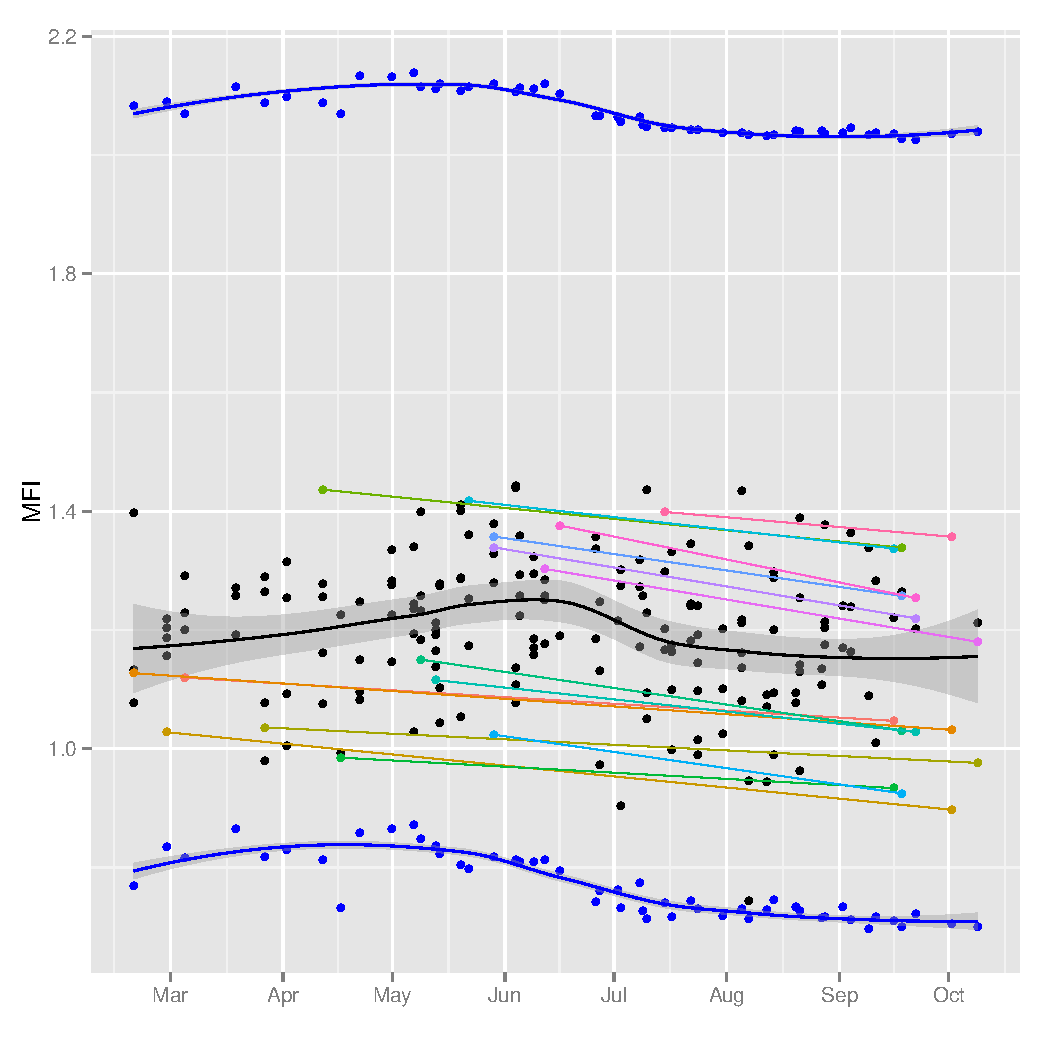
\includegraphics[scale=.5]{IL2RA/figures/CD25-MFI-time-effect-repeatability.pdf}
        \caption{Unormalised.}
    \end{subfigure}
    ~
    \begin{subfigure}[b]{.5\textwidth}
        \centering
        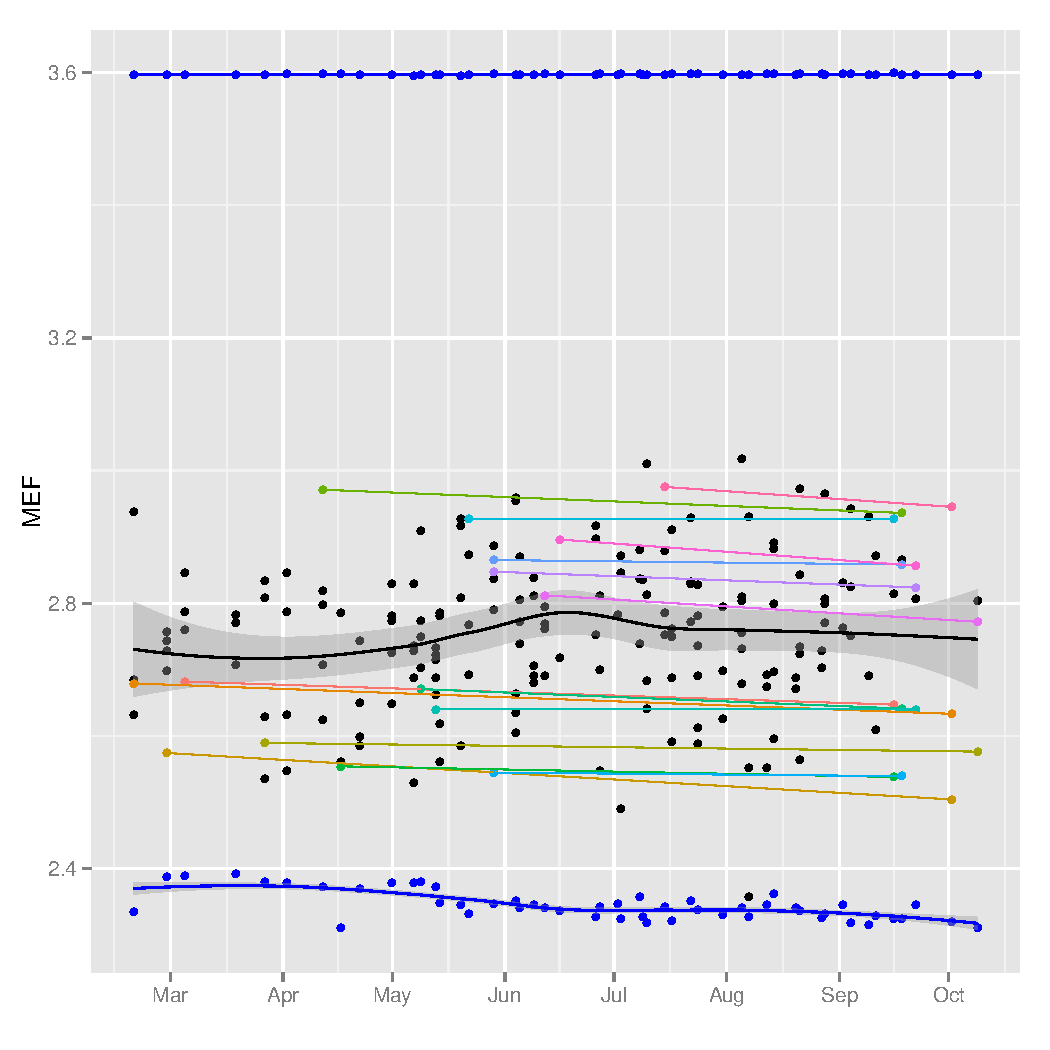
\includegraphics[scale=.5]{IL2RA/figures/CD25-MFI-time-effect-beads-normalised.pdf}
        \caption{Normalised}
    \end{subfigure}
    ~
    \begin{subfigure}[b]{.5\textwidth}
        \centering
        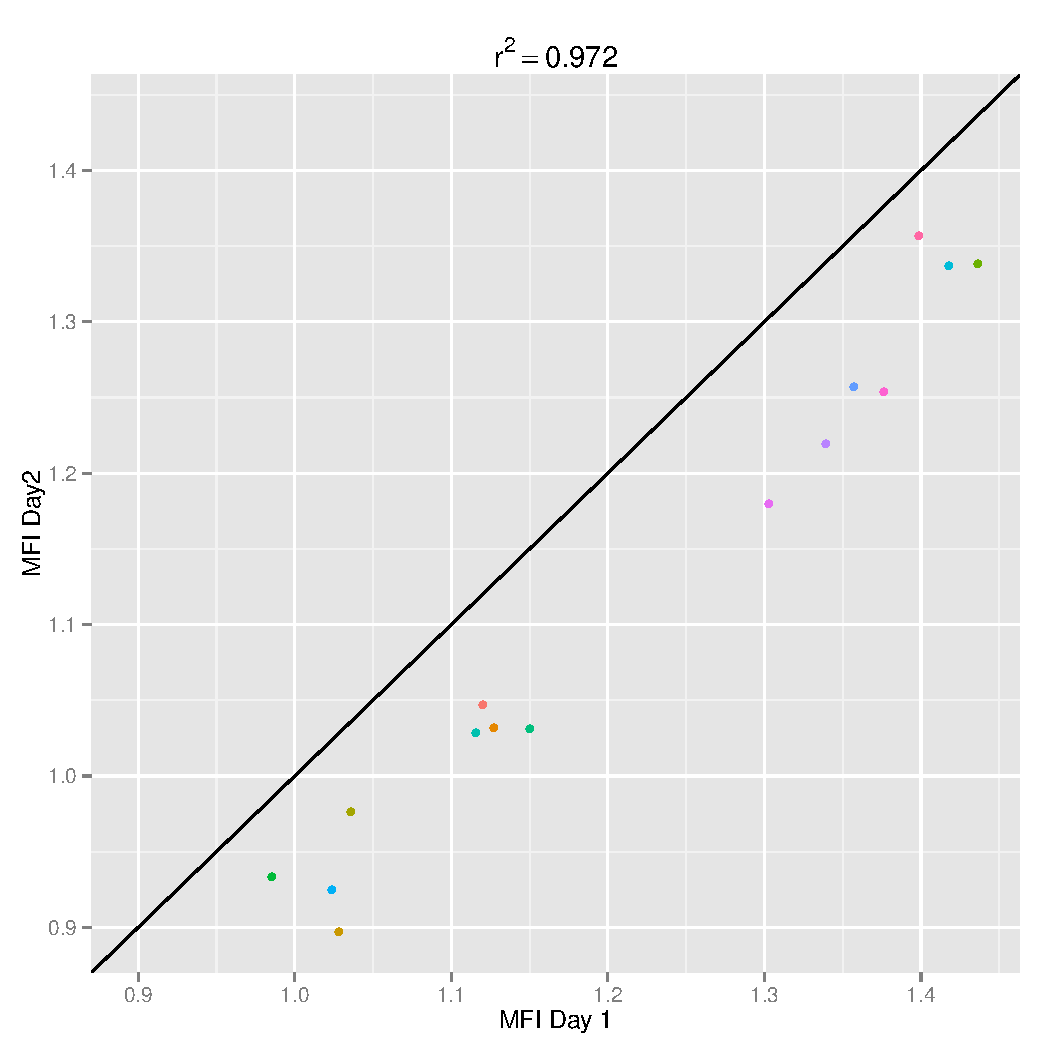
\includegraphics[scale=.75]{IL2RA/figures/CD25-MFI-repeatability.pdf}
        \caption{Unormalised: $R^2=0.629$}
    \end{subfigure}
    ~
    \begin{subfigure}[b]{.5\textwidth}
        \centering
        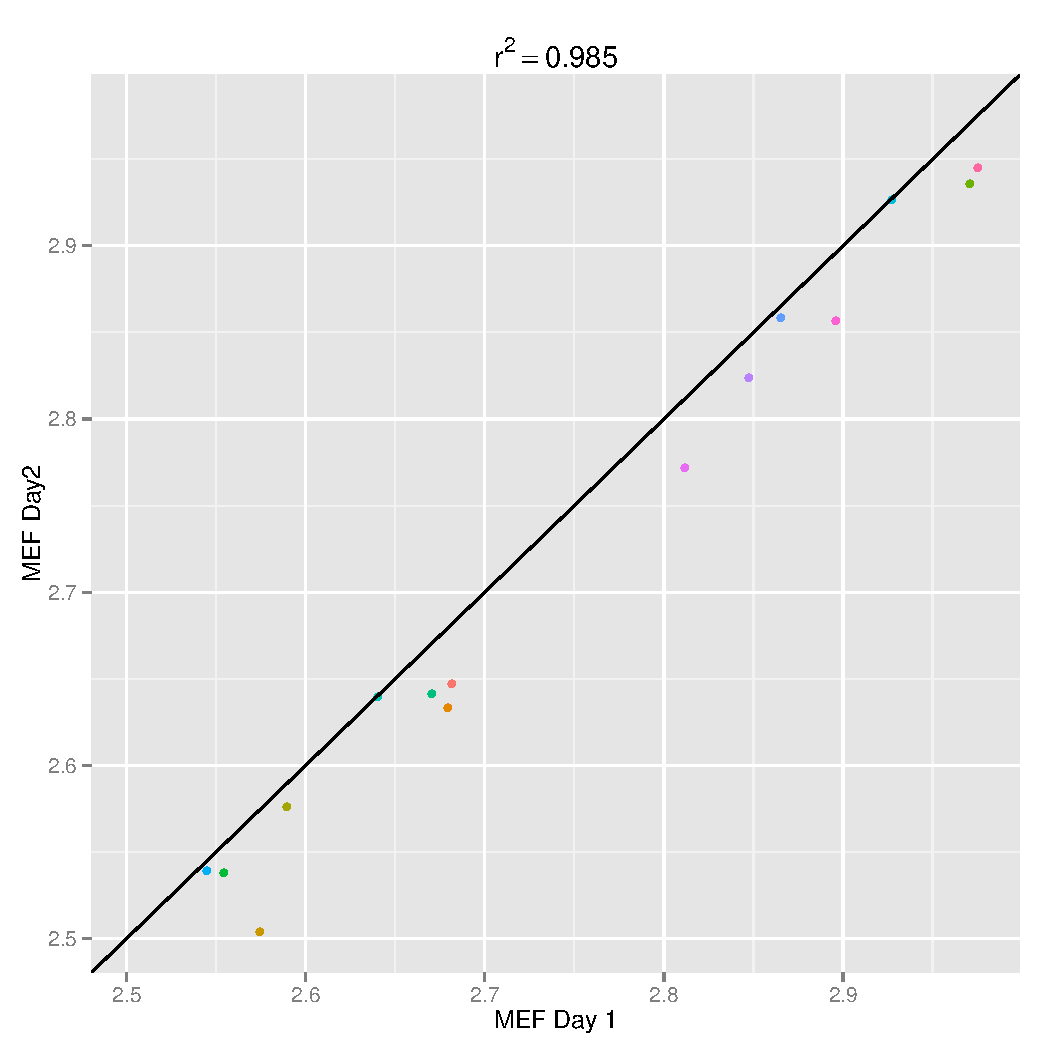
\includegraphics[scale=.75]{IL2RA/figures/CD25-MFI-beads-normalised.pdf}
        \caption{Normalised: $R^2=0.937$}
    \end{subfigure}
%\end{center}
    \caption{ \label{figure:CD25-MFI-beads-normalised.pdf}
\textbf{Bead normalisation partly corrects for long term time effect in CD25 MFI of the memory cell population.}
In \textbf{(a)} and \textbf{(b)}, the blue points represent the MFIs of the bead populations, in black the MFIs of the memory cell populations.
A loess is fitted to the MFIs of the beads and memory cells.
The points joined by lines are MFIs from recalled individuals.
The normalisation step involves aligning the peaks of the two bead populations across days to the overall mean of each of the populations (the dashed blue).
The normalisation improves the repeatability of the MFI in recalled individuals from $R^2=0.629$ \textbf{(c)} to $R^2=0.937$ \textbf{(d)}.
}
\end{figure}




 
%\chapter{\label{maths}{Maths}}
%\input{Appendix/maths} 
\end{appendices}


